	\chapter{Présentation du business model}
		\section{Présentation de la stratégie de l'entreprise}
			% Où voulez vous aller ? mener le marché . innover . suivre une idée existante ?
			Le but de \K{} est d'apporter une solution aux petites entreprises, à leurs portée.
			Nous avons a coeur de promouvoir l'écologie, a travers des circuits régionnaux et la proximité entre les vendeurs et les clients.
			C'est pour cela que notre offre vise a aider les petites entreprise, qui sont les plus proches des clients et des utilisateurs finaux.
			Nous souhaitons donc innover pour ces interlocuteurs en leurs offant un produit gratuit, simple et efficace.
			% Comment pensez vous y parvenir ? innover et trouver quelque chose que les autres n'ont pas ? monopole ?
			Comme dit précédement, nous comptons nous insérer sur le marché avec un produit fait pour ces entreprises.
			Ainsi, elles ne devront plus dépendre d'un logiciel très couteux fait pour des structures énormes,
			ni sur des tableurs créés en interne et peu fiables.
			C'est cette échelle humaine, dont les autres logiciels ne disposent pas, qui est notre atout majeur pour notre insertion dans le marché.
			
		\section{Présentation de l'organisation de l'entreprise}
			% Comment sont affectées les fonctions dans l'entreprise ? détailler acquisition / production / distribution / administration
			Le Conseil d'Administration, constitué de tout les associés, se réunira tout les mois.\\
			Son rôle sera de décider des objectifs de l'entreprise a court terme, a savoir le mois suivant.
			Dans une première partie, la rétrospective, 
			on y évoquera les soucis et les solutions trouvés dans le mois précédent. On modifiera ensuite le cas échéant nos pratiques afin
			d'améliorer le confort de tous.
			Le CA se penchera enfin sur les finances, et recalculera si besoin est le taux horaire des associés et des salariés (qui est unique)\\
			Tout les 6 mois, le conseil se réunira exceptionellement pour réfléchir a la politique à long terme de l'entreprise.
			Cette session sera uniquement dédié à ce but, et commencera par une retrospective des 6 derniers mois
			avant les discutions et l'établissement d'un but a atteindre.
			Le CA nommera, tout les 6 mois, un président, un directeur, un secrétaire et un trésorier pour les 6 mois a venir.
			Ces mandats ne seront ni cumulables ni reconduisibles sur deux semestres consecutifs, forçant chacun a s'investir dans l'entreprise. \\
			Il sera aussi possible, a tout moment et pour tout salartié de l'entreprise, de demander une session extraordinaire.

			De part notre position dans le secteur tertiaire, notre société n'a pas de structure formelle pour l'acquisition.
			Nous n'avons pas de matière premier à acheter.

			Les investissements et les  achats de fourniture  seront décidés en Conseil d'aministration,

			Pour ce qui est de la production, un serveur interne a l'entreprise nous permettra de centraliser le travail et de nous connecter à nos stations
			depuis n'importe quel ordinateur de la société. Nous disposerons aussi de postes personnels afin de développer nos logiciels. \\
			\clem{}, \soum{} et \drm{} S'occuperons du développement du logiciel tandis que \ben{} et \bonte{} rédigerons l'aide et les tutoriels, tout en testant et 
			validant les calculs effectués par les logiciels.

			La distribution est quand à elle gérée par \bonte{} et \ben{}. Ils s'occuperons de prospecter les clients, prendre contact avec les annonceurs
			et répondre au service après vente qu'ils pourront, le cas échéant, transférer à l'un des developpeurs.

			Du côté administratif, notre status de SCOP et notre faible nombre nous permettrons de gérer la plupart des cas en Conseil d'Administration.
			De plus, nous nommerons tout les mois un responsable chargé de régler les problèmes anodins tels que, par exemple, une coupure d'accès à internet ou
			l'approvisionnement de la cafetière.
			
			% Présenter un organigramme de l'entreprise
		\section{Organigramme de l'entreprise}
			Comme nous avons l'intention de nous implanter avec un statut de SCOP, nous serons tous associés et nous aurons 
			tous les cinq le même poids lors des votes au conseil d'administration. L'organigramme de \K{} peut donc se
			représenter selon la figure \ref{fig:org}.
			\begin{figure}[h]
			  \begin{center}
				% Graphic for TeX using PGF
% Title: /home/mathieu/businessPlanKlimasoft/includes/Organigramme.dia
% Creator: Dia v0.97.1
% CreationDate: Sat Mar 24 16:53:15 2012
% For: mathieu
% \usepackage{tikz}
% The following commands are not supported in PSTricks at present
% We define them conditionally, so when they are implemented,
% this pgf file will use them.
\ifx\du\undefined
  \newlength{\du}
\fi
\setlength{\du}{15\unitlength}
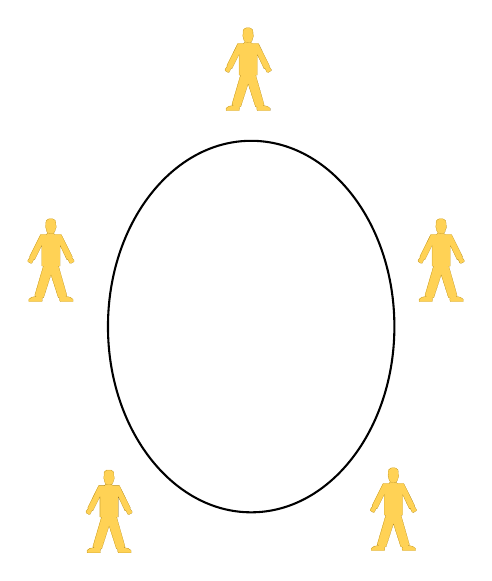
\begin{tikzpicture}
\pgftransformxscale{1.000000}
\pgftransformyscale{-1.000000}
\definecolor{dialinecolor}{rgb}{0.000000, 0.000000, 0.000000}
\pgfsetstrokecolor{dialinecolor}
\definecolor{dialinecolor}{rgb}{1.000000, 1.000000, 1.000000}
\pgfsetfillcolor{dialinecolor}
\definecolor{dialinecolor}{rgb}{1.000000, 1.000000, 1.000000}
\pgfsetfillcolor{dialinecolor}
\pgfpathellipse{\pgfpoint{37.959375\du}{9.878125\du}}{\pgfpoint{3.450000\du}{0\du}}{\pgfpoint{0\du}{4.475000\du}}
\pgfusepath{fill}
\pgfsetlinewidth{0.050000\du}
\pgfsetdash{}{0pt}
\pgfsetdash{}{0pt}
\definecolor{dialinecolor}{rgb}{0.000000, 0.000000, 0.000000}
\pgfsetstrokecolor{dialinecolor}
\pgfpathellipse{\pgfpoint{37.959375\du}{9.878125\du}}{\pgfpoint{3.450000\du}{0\du}}{\pgfpoint{0\du}{4.475000\du}}
\pgfusepath{stroke}
\pgfsetlinewidth{0.050000\du}
\pgfsetdash{}{0pt}
\pgfsetdash{}{0pt}
\pgfsetbuttcap
\pgfsetmiterjoin
\pgfsetlinewidth{0.000500\du}
\pgfsetbuttcap
\pgfsetmiterjoin
\pgfsetdash{}{0pt}
\definecolor{dialinecolor}{rgb}{1.000000, 0.823529, 0.333333}
\pgfsetfillcolor{dialinecolor}
\pgfpathmoveto{\pgfpoint{37.367856\du}{3.584915\du}}
\pgfpathlineto{\pgfpoint{37.380790\du}{3.597287\du}}
\pgfpathlineto{\pgfpoint{37.325680\du}{3.677984\du}}
\pgfpathlineto{\pgfpoint{37.325680\du}{3.708914\du}}
\pgfpathlineto{\pgfpoint{37.398785\du}{3.752496\du}}
\pgfpathlineto{\pgfpoint{37.423529\du}{3.746310\du}}
\pgfpathlineto{\pgfpoint{37.472172\du}{3.646774\du}}
\pgfpathlineto{\pgfpoint{37.490448\du}{3.659146\du}}
\pgfpathlineto{\pgfpoint{37.661403\du}{3.317799\du}}
\pgfpathlineto{\pgfpoint{37.661403\du}{3.814636\du}}
\pgfpathlineto{\pgfpoint{37.697956\du}{3.814636\du}}
\pgfpathlineto{\pgfpoint{37.490448\du}{4.522635\du}}
\pgfpathlineto{\pgfpoint{37.521378\du}{4.547660\du}}
\pgfpathlineto{\pgfpoint{37.417062\du}{4.566217\du}}
\pgfpathlineto{\pgfpoint{37.350142\du}{4.615985\du}}
\pgfpathlineto{\pgfpoint{37.350142\du}{4.671658\du}}
\pgfpathlineto{\pgfpoint{37.667589\du}{4.671658\du}}
\pgfpathlineto{\pgfpoint{37.673494\du}{4.622171\du}}
\pgfpathlineto{\pgfpoint{37.667589\du}{4.584775\du}}
\pgfpathlineto{\pgfpoint{37.704142\du}{4.578589\du}}
\pgfpathlineto{\pgfpoint{37.881001\du}{4.025798\du}}
\pgfpathlineto{\pgfpoint{38.058423\du}{4.578589\du}}
\pgfpathlineto{\pgfpoint{38.094975\du}{4.584775\du}}
\pgfpathlineto{\pgfpoint{38.088508\du}{4.628357\du}}
\pgfpathlineto{\pgfpoint{38.100880\du}{4.671658\du}}
\pgfpathlineto{\pgfpoint{38.412422\du}{4.671658\du}}
\pgfpathlineto{\pgfpoint{38.412422\du}{4.615985\du}}
\pgfpathlineto{\pgfpoint{38.344940\du}{4.566217\du}}
\pgfpathlineto{\pgfpoint{38.241186\du}{4.547660\du}}
\pgfpathlineto{\pgfpoint{38.265930\du}{4.522635\du}}
\pgfpathlineto{\pgfpoint{38.064046\du}{3.814636\du}}
\pgfpathlineto{\pgfpoint{38.100880\du}{3.814636\du}}
\pgfpathlineto{\pgfpoint{38.100880\du}{3.317799\du}}
\pgfpathlineto{\pgfpoint{38.265930\du}{3.665613\du}}
\pgfpathlineto{\pgfpoint{38.284487\du}{3.646774\du}}
\pgfpathlineto{\pgfpoint{38.332850\du}{3.746310\du}}
\pgfpathlineto{\pgfpoint{38.363779\du}{3.752496\du}}
\pgfpathlineto{\pgfpoint{38.436603\du}{3.708914\du}}
\pgfpathlineto{\pgfpoint{38.436603\du}{3.677984\du}}
\pgfpathlineto{\pgfpoint{38.381774\du}{3.597287\du}}
\pgfpathlineto{\pgfpoint{38.394146\du}{3.584915\du}}
\pgfpathlineto{\pgfpoint{38.131528\du}{3.056868\du}}
\pgfpathlineto{\pgfpoint{37.979131\du}{3.056868\du}}
\pgfpathlineto{\pgfpoint{37.930207\du}{3.007100\du}}
\pgfpathlineto{\pgfpoint{37.814081\du}{3.007100\du}}
\pgfpathlineto{\pgfpoint{37.771343\du}{3.056868\du}}
\pgfpathlineto{\pgfpoint{37.631036\du}{3.056868\du}}
\pgfpathlineto{\pgfpoint{37.367856\du}{3.584915\du}}
\pgfusepath{fill}
\pgfsetbuttcap
\pgfsetmiterjoin
\pgfsetdash{}{0pt}
\definecolor{dialinecolor}{rgb}{1.000000, 0.823529, 0.333333}
\pgfsetfillcolor{dialinecolor}
\pgfpathmoveto{\pgfpoint{37.374604\du}{3.590820\du}}
\pgfpathlineto{\pgfpoint{37.386695\du}{3.603473\du}}
\pgfpathlineto{\pgfpoint{37.331866\du}{3.684170\du}}
\pgfpathlineto{\pgfpoint{37.331866\du}{3.715381\du}}
\pgfpathlineto{\pgfpoint{37.404690\du}{3.758682\du}}
\pgfpathlineto{\pgfpoint{37.429152\du}{3.752496\du}}
\pgfpathlineto{\pgfpoint{37.478358\du}{3.652960\du}}
\pgfpathlineto{\pgfpoint{37.496353\du}{3.665613\du}}
\pgfpathlineto{\pgfpoint{37.667589\du}{3.323985\du}}
\pgfpathlineto{\pgfpoint{37.667589\du}{3.820821\du}}
\pgfpathlineto{\pgfpoint{37.704142\du}{3.820821\du}}
\pgfpathlineto{\pgfpoint{37.496353\du}{4.529102\du}}
\pgfpathlineto{\pgfpoint{37.527001\du}{4.553846\du}}
\pgfpathlineto{\pgfpoint{37.423529\du}{4.572684\du}}
\pgfpathlineto{\pgfpoint{37.355765\du}{4.622171\du}}
\pgfpathlineto{\pgfpoint{37.355765\du}{4.678125\du}}
\pgfpathlineto{\pgfpoint{37.673494\du}{4.678125\du}}
\pgfpathlineto{\pgfpoint{37.679679\du}{4.628357\du}}
\pgfpathlineto{\pgfpoint{37.673494\du}{4.590961\du}}
\pgfpathlineto{\pgfpoint{37.710327\du}{4.584775\du}}
\pgfpathlineto{\pgfpoint{37.887468\du}{4.032265\du}}
\pgfpathlineto{\pgfpoint{38.064046\du}{4.584775\du}}
\pgfpathlineto{\pgfpoint{38.100880\du}{4.590961\du}}
\pgfpathlineto{\pgfpoint{38.094975\du}{4.634543\du}}
\pgfpathlineto{\pgfpoint{38.107066\du}{4.678125\du}}
\pgfpathlineto{\pgfpoint{38.418608\du}{4.678125\du}}
\pgfpathlineto{\pgfpoint{38.418608\du}{4.622171\du}}
\pgfpathlineto{\pgfpoint{38.351407\du}{4.572684\du}}
\pgfpathlineto{\pgfpoint{38.247654\du}{4.553846\du}}
\pgfpathlineto{\pgfpoint{38.272116\du}{4.529102\du}}
\pgfpathlineto{\pgfpoint{38.070794\du}{3.820821\du}}
\pgfpathlineto{\pgfpoint{38.107066\du}{3.820821\du}}
\pgfpathlineto{\pgfpoint{38.107066\du}{3.323985\du}}
\pgfpathlineto{\pgfpoint{38.272116\du}{3.671799\du}}
\pgfpathlineto{\pgfpoint{38.290392\du}{3.652960\du}}
\pgfpathlineto{\pgfpoint{38.339317\du}{3.752496\du}}
\pgfpathlineto{\pgfpoint{38.369684\du}{3.758682\du}}
\pgfpathlineto{\pgfpoint{38.443070\du}{3.715381\du}}
\pgfpathlineto{\pgfpoint{38.443070\du}{3.684170\du}}
\pgfpathlineto{\pgfpoint{38.387960\du}{3.603473\du}}
\pgfpathlineto{\pgfpoint{38.400332\du}{3.590820\du}}
\pgfpathlineto{\pgfpoint{38.137714\du}{3.062773\du}}
\pgfpathlineto{\pgfpoint{37.984755\du}{3.062773\du}}
\pgfpathlineto{\pgfpoint{37.936111\du}{3.013567\du}}
\pgfpathlineto{\pgfpoint{37.820267\du}{3.013567\du}}
\pgfpathlineto{\pgfpoint{37.777247\du}{3.062773\du}}
\pgfpathlineto{\pgfpoint{37.636660\du}{3.062773\du}}
\pgfpathlineto{\pgfpoint{37.374604\du}{3.590820\du}}
\pgfusepath{fill}
\pgfsetbuttcap
\pgfsetmiterjoin
\pgfsetdash{}{0pt}
\definecolor{dialinecolor}{rgb}{0.501961, 0.364706, 0.000000}
\pgfsetstrokecolor{dialinecolor}
\pgfpathmoveto{\pgfpoint{37.374604\du}{3.590820\du}}
\pgfpathlineto{\pgfpoint{37.386695\du}{3.603473\du}}
\pgfpathlineto{\pgfpoint{37.331866\du}{3.684170\du}}
\pgfpathlineto{\pgfpoint{37.331866\du}{3.715381\du}}
\pgfpathlineto{\pgfpoint{37.404690\du}{3.758682\du}}
\pgfpathlineto{\pgfpoint{37.429152\du}{3.752496\du}}
\pgfpathlineto{\pgfpoint{37.478358\du}{3.652960\du}}
\pgfpathlineto{\pgfpoint{37.496353\du}{3.665613\du}}
\pgfpathlineto{\pgfpoint{37.667589\du}{3.323985\du}}
\pgfpathlineto{\pgfpoint{37.667589\du}{3.820821\du}}
\pgfpathlineto{\pgfpoint{37.704142\du}{3.820821\du}}
\pgfpathlineto{\pgfpoint{37.496353\du}{4.529102\du}}
\pgfpathlineto{\pgfpoint{37.527001\du}{4.553846\du}}
\pgfpathlineto{\pgfpoint{37.423529\du}{4.572684\du}}
\pgfpathlineto{\pgfpoint{37.355765\du}{4.622171\du}}
\pgfpathlineto{\pgfpoint{37.355765\du}{4.678125\du}}
\pgfpathlineto{\pgfpoint{37.673494\du}{4.678125\du}}
\pgfpathlineto{\pgfpoint{37.679679\du}{4.628357\du}}
\pgfpathlineto{\pgfpoint{37.673494\du}{4.590961\du}}
\pgfpathlineto{\pgfpoint{37.710327\du}{4.584775\du}}
\pgfpathlineto{\pgfpoint{37.887468\du}{4.032265\du}}
\pgfpathlineto{\pgfpoint{38.064046\du}{4.584775\du}}
\pgfpathlineto{\pgfpoint{38.100880\du}{4.590961\du}}
\pgfpathlineto{\pgfpoint{38.094975\du}{4.634543\du}}
\pgfpathlineto{\pgfpoint{38.107066\du}{4.678125\du}}
\pgfpathlineto{\pgfpoint{38.418608\du}{4.678125\du}}
\pgfpathlineto{\pgfpoint{38.418608\du}{4.622171\du}}
\pgfpathlineto{\pgfpoint{38.351407\du}{4.572684\du}}
\pgfpathlineto{\pgfpoint{38.247654\du}{4.553846\du}}
\pgfpathlineto{\pgfpoint{38.272116\du}{4.529102\du}}
\pgfpathlineto{\pgfpoint{38.070794\du}{3.820821\du}}
\pgfpathlineto{\pgfpoint{38.107066\du}{3.820821\du}}
\pgfpathlineto{\pgfpoint{38.107066\du}{3.323985\du}}
\pgfpathlineto{\pgfpoint{38.272116\du}{3.671799\du}}
\pgfpathlineto{\pgfpoint{38.290392\du}{3.652960\du}}
\pgfpathlineto{\pgfpoint{38.339317\du}{3.752496\du}}
\pgfpathlineto{\pgfpoint{38.369684\du}{3.758682\du}}
\pgfpathlineto{\pgfpoint{38.443070\du}{3.715381\du}}
\pgfpathlineto{\pgfpoint{38.443070\du}{3.684170\du}}
\pgfpathlineto{\pgfpoint{38.387960\du}{3.603473\du}}
\pgfpathlineto{\pgfpoint{38.400332\du}{3.590820\du}}
\pgfpathlineto{\pgfpoint{38.137714\du}{3.062773\du}}
\pgfpathlineto{\pgfpoint{37.984755\du}{3.062773\du}}
\pgfpathlineto{\pgfpoint{37.936111\du}{3.013567\du}}
\pgfpathlineto{\pgfpoint{37.820267\du}{3.013567\du}}
\pgfpathlineto{\pgfpoint{37.777247\du}{3.062773\du}}
\pgfpathlineto{\pgfpoint{37.636660\du}{3.062773\du}}
\pgfpathlineto{\pgfpoint{37.374604\du}{3.590820\du}}
\pgfusepath{stroke}
\pgfsetbuttcap
\pgfsetmiterjoin
\pgfsetdash{}{0pt}
\definecolor{dialinecolor}{rgb}{1.000000, 0.823529, 0.333333}
\pgfsetfillcolor{dialinecolor}
\pgfpathmoveto{\pgfpoint{37.911930\du}{2.678125\du}}
\pgfpathlineto{\pgfpoint{37.844729\du}{2.678125\du}}
\pgfpathlineto{\pgfpoint{37.814081\du}{2.684030\du}}
\pgfpathlineto{\pgfpoint{37.764875\du}{2.727612\du}}
\pgfpathlineto{\pgfpoint{37.759252\du}{2.771194\du}}
\pgfpathlineto{\pgfpoint{37.759252\du}{2.826867\du}}
\pgfpathlineto{\pgfpoint{37.752785\du}{2.851891\du}}
\pgfpathlineto{\pgfpoint{37.752785\du}{2.876635\du}}
\pgfpathlineto{\pgfpoint{37.783433\du}{2.988261\du}}
\pgfpathlineto{\pgfpoint{37.814081\du}{3.019472\du}}
\pgfpathlineto{\pgfpoint{37.881001\du}{3.031844\du}}
\pgfpathlineto{\pgfpoint{37.942297\du}{3.019472\du}}
\pgfpathlineto{\pgfpoint{37.972383\du}{2.988261\du}}
\pgfpathlineto{\pgfpoint{37.997126\du}{2.913750\du}}
\pgfpathlineto{\pgfpoint{38.009217\du}{2.876635\du}}
\pgfpathlineto{\pgfpoint{38.009217\du}{2.851891\du}}
\pgfpathlineto{\pgfpoint{37.997126\du}{2.826867\du}}
\pgfpathlineto{\pgfpoint{37.997126\du}{2.771194\du}}
\pgfpathlineto{\pgfpoint{37.991503\du}{2.727612\du}}
\pgfpathlineto{\pgfpoint{37.942297\du}{2.684030\du}}
\pgfpathlineto{\pgfpoint{37.911930\du}{2.678125\du}}
\pgfusepath{fill}
\pgfsetbuttcap
\pgfsetmiterjoin
\pgfsetdash{}{0pt}
\definecolor{dialinecolor}{rgb}{1.000000, 0.823529, 0.333333}
\pgfsetfillcolor{dialinecolor}
\pgfpathmoveto{\pgfpoint{37.917835\du}{2.684030\du}}
\pgfpathlineto{\pgfpoint{37.850634\du}{2.684030\du}}
\pgfpathlineto{\pgfpoint{37.820267\du}{2.690216\du}}
\pgfpathlineto{\pgfpoint{37.771343\du}{2.733517\du}}
\pgfpathlineto{\pgfpoint{37.764875\du}{2.777099\du}}
\pgfpathlineto{\pgfpoint{37.764875\du}{2.833053\du}}
\pgfpathlineto{\pgfpoint{37.759252\du}{2.857796\du}}
\pgfpathlineto{\pgfpoint{37.759252\du}{2.882821\du}}
\pgfpathlineto{\pgfpoint{37.789619\du}{2.994447\du}}
\pgfpathlineto{\pgfpoint{37.820267\du}{3.025939\du}}
\pgfpathlineto{\pgfpoint{37.887468\du}{3.038311\du}}
\pgfpathlineto{\pgfpoint{37.948764\du}{3.025939\du}}
\pgfpathlineto{\pgfpoint{37.979131\du}{2.994447\du}}
\pgfpathlineto{\pgfpoint{38.003312\du}{2.919936\du}}
\pgfpathlineto{\pgfpoint{38.015684\du}{2.882821\du}}
\pgfpathlineto{\pgfpoint{38.015684\du}{2.857796\du}}
\pgfpathlineto{\pgfpoint{38.003312\du}{2.833053\du}}
\pgfpathlineto{\pgfpoint{38.003312\du}{2.777099\du}}
\pgfpathlineto{\pgfpoint{37.997126\du}{2.733517\du}}
\pgfpathlineto{\pgfpoint{37.948764\du}{2.690216\du}}
\pgfpathlineto{\pgfpoint{37.917835\du}{2.684030\du}}
\pgfusepath{fill}
\pgfsetbuttcap
\pgfsetmiterjoin
\pgfsetdash{}{0pt}
\definecolor{dialinecolor}{rgb}{0.501961, 0.364706, 0.000000}
\pgfsetstrokecolor{dialinecolor}
\pgfpathmoveto{\pgfpoint{37.917835\du}{2.684030\du}}
\pgfpathlineto{\pgfpoint{37.850634\du}{2.684030\du}}
\pgfpathlineto{\pgfpoint{37.820267\du}{2.690216\du}}
\pgfpathlineto{\pgfpoint{37.771343\du}{2.733517\du}}
\pgfpathlineto{\pgfpoint{37.764875\du}{2.777099\du}}
\pgfpathlineto{\pgfpoint{37.764875\du}{2.833053\du}}
\pgfpathlineto{\pgfpoint{37.759252\du}{2.857796\du}}
\pgfpathlineto{\pgfpoint{37.759252\du}{2.882821\du}}
\pgfpathlineto{\pgfpoint{37.789619\du}{2.994447\du}}
\pgfpathlineto{\pgfpoint{37.820267\du}{3.025939\du}}
\pgfpathlineto{\pgfpoint{37.887468\du}{3.038311\du}}
\pgfpathlineto{\pgfpoint{37.948764\du}{3.025939\du}}
\pgfpathlineto{\pgfpoint{37.979131\du}{2.994447\du}}
\pgfpathlineto{\pgfpoint{38.003312\du}{2.919936\du}}
\pgfpathlineto{\pgfpoint{38.015684\du}{2.882821\du}}
\pgfpathlineto{\pgfpoint{38.015684\du}{2.857796\du}}
\pgfpathlineto{\pgfpoint{38.003312\du}{2.833053\du}}
\pgfpathlineto{\pgfpoint{38.003312\du}{2.777099\du}}
\pgfpathlineto{\pgfpoint{37.997126\du}{2.733517\du}}
\pgfpathlineto{\pgfpoint{37.948764\du}{2.690216\du}}
\pgfpathlineto{\pgfpoint{37.917835\du}{2.684030\du}}
\pgfusepath{stroke}
\pgfsetlinewidth{0.050000\du}
\pgfsetdash{}{0pt}
\pgfsetdash{}{0pt}
\pgfsetbuttcap
\pgfsetmiterjoin
\pgfsetlinewidth{0.000500\du}
\pgfsetbuttcap
\pgfsetmiterjoin
\pgfsetdash{}{0pt}
\definecolor{dialinecolor}{rgb}{1.000000, 0.823529, 0.333333}
\pgfsetfillcolor{dialinecolor}
\pgfpathmoveto{\pgfpoint{42.017856\du}{8.184915\du}}
\pgfpathlineto{\pgfpoint{42.030790\du}{8.197287\du}}
\pgfpathlineto{\pgfpoint{41.975680\du}{8.277984\du}}
\pgfpathlineto{\pgfpoint{41.975680\du}{8.308914\du}}
\pgfpathlineto{\pgfpoint{42.048785\du}{8.352496\du}}
\pgfpathlineto{\pgfpoint{42.073529\du}{8.346310\du}}
\pgfpathlineto{\pgfpoint{42.122172\du}{8.246774\du}}
\pgfpathlineto{\pgfpoint{42.140448\du}{8.259146\du}}
\pgfpathlineto{\pgfpoint{42.311403\du}{7.917799\du}}
\pgfpathlineto{\pgfpoint{42.311403\du}{8.414636\du}}
\pgfpathlineto{\pgfpoint{42.347956\du}{8.414636\du}}
\pgfpathlineto{\pgfpoint{42.140448\du}{9.122635\du}}
\pgfpathlineto{\pgfpoint{42.171378\du}{9.147660\du}}
\pgfpathlineto{\pgfpoint{42.067062\du}{9.166217\du}}
\pgfpathlineto{\pgfpoint{42.000142\du}{9.215985\du}}
\pgfpathlineto{\pgfpoint{42.000142\du}{9.271658\du}}
\pgfpathlineto{\pgfpoint{42.317589\du}{9.271658\du}}
\pgfpathlineto{\pgfpoint{42.323494\du}{9.222171\du}}
\pgfpathlineto{\pgfpoint{42.317589\du}{9.184775\du}}
\pgfpathlineto{\pgfpoint{42.354142\du}{9.178589\du}}
\pgfpathlineto{\pgfpoint{42.531001\du}{8.625798\du}}
\pgfpathlineto{\pgfpoint{42.708423\du}{9.178589\du}}
\pgfpathlineto{\pgfpoint{42.744975\du}{9.184775\du}}
\pgfpathlineto{\pgfpoint{42.738508\du}{9.228357\du}}
\pgfpathlineto{\pgfpoint{42.750880\du}{9.271658\du}}
\pgfpathlineto{\pgfpoint{43.062422\du}{9.271658\du}}
\pgfpathlineto{\pgfpoint{43.062422\du}{9.215985\du}}
\pgfpathlineto{\pgfpoint{42.994940\du}{9.166217\du}}
\pgfpathlineto{\pgfpoint{42.891186\du}{9.147660\du}}
\pgfpathlineto{\pgfpoint{42.915930\du}{9.122635\du}}
\pgfpathlineto{\pgfpoint{42.714046\du}{8.414636\du}}
\pgfpathlineto{\pgfpoint{42.750880\du}{8.414636\du}}
\pgfpathlineto{\pgfpoint{42.750880\du}{7.917799\du}}
\pgfpathlineto{\pgfpoint{42.915930\du}{8.265613\du}}
\pgfpathlineto{\pgfpoint{42.934487\du}{8.246774\du}}
\pgfpathlineto{\pgfpoint{42.982850\du}{8.346310\du}}
\pgfpathlineto{\pgfpoint{43.013779\du}{8.352496\du}}
\pgfpathlineto{\pgfpoint{43.086603\du}{8.308914\du}}
\pgfpathlineto{\pgfpoint{43.086603\du}{8.277984\du}}
\pgfpathlineto{\pgfpoint{43.031774\du}{8.197287\du}}
\pgfpathlineto{\pgfpoint{43.044146\du}{8.184915\du}}
\pgfpathlineto{\pgfpoint{42.781528\du}{7.656868\du}}
\pgfpathlineto{\pgfpoint{42.629131\du}{7.656868\du}}
\pgfpathlineto{\pgfpoint{42.580207\du}{7.607100\du}}
\pgfpathlineto{\pgfpoint{42.464081\du}{7.607100\du}}
\pgfpathlineto{\pgfpoint{42.421343\du}{7.656868\du}}
\pgfpathlineto{\pgfpoint{42.281036\du}{7.656868\du}}
\pgfpathlineto{\pgfpoint{42.017856\du}{8.184915\du}}
\pgfusepath{fill}
\pgfsetbuttcap
\pgfsetmiterjoin
\pgfsetdash{}{0pt}
\definecolor{dialinecolor}{rgb}{1.000000, 0.823529, 0.333333}
\pgfsetfillcolor{dialinecolor}
\pgfpathmoveto{\pgfpoint{42.024604\du}{8.190820\du}}
\pgfpathlineto{\pgfpoint{42.036695\du}{8.203473\du}}
\pgfpathlineto{\pgfpoint{41.981866\du}{8.284170\du}}
\pgfpathlineto{\pgfpoint{41.981866\du}{8.315381\du}}
\pgfpathlineto{\pgfpoint{42.054690\du}{8.358682\du}}
\pgfpathlineto{\pgfpoint{42.079152\du}{8.352496\du}}
\pgfpathlineto{\pgfpoint{42.128358\du}{8.252960\du}}
\pgfpathlineto{\pgfpoint{42.146353\du}{8.265613\du}}
\pgfpathlineto{\pgfpoint{42.317589\du}{7.923985\du}}
\pgfpathlineto{\pgfpoint{42.317589\du}{8.420821\du}}
\pgfpathlineto{\pgfpoint{42.354142\du}{8.420821\du}}
\pgfpathlineto{\pgfpoint{42.146353\du}{9.129102\du}}
\pgfpathlineto{\pgfpoint{42.177001\du}{9.153846\du}}
\pgfpathlineto{\pgfpoint{42.073529\du}{9.172684\du}}
\pgfpathlineto{\pgfpoint{42.005765\du}{9.222171\du}}
\pgfpathlineto{\pgfpoint{42.005765\du}{9.278125\du}}
\pgfpathlineto{\pgfpoint{42.323494\du}{9.278125\du}}
\pgfpathlineto{\pgfpoint{42.329679\du}{9.228357\du}}
\pgfpathlineto{\pgfpoint{42.323494\du}{9.190961\du}}
\pgfpathlineto{\pgfpoint{42.360327\du}{9.184775\du}}
\pgfpathlineto{\pgfpoint{42.537468\du}{8.632265\du}}
\pgfpathlineto{\pgfpoint{42.714046\du}{9.184775\du}}
\pgfpathlineto{\pgfpoint{42.750880\du}{9.190961\du}}
\pgfpathlineto{\pgfpoint{42.744975\du}{9.234543\du}}
\pgfpathlineto{\pgfpoint{42.757066\du}{9.278125\du}}
\pgfpathlineto{\pgfpoint{43.068608\du}{9.278125\du}}
\pgfpathlineto{\pgfpoint{43.068608\du}{9.222171\du}}
\pgfpathlineto{\pgfpoint{43.001407\du}{9.172684\du}}
\pgfpathlineto{\pgfpoint{42.897654\du}{9.153846\du}}
\pgfpathlineto{\pgfpoint{42.922116\du}{9.129102\du}}
\pgfpathlineto{\pgfpoint{42.720794\du}{8.420821\du}}
\pgfpathlineto{\pgfpoint{42.757066\du}{8.420821\du}}
\pgfpathlineto{\pgfpoint{42.757066\du}{7.923985\du}}
\pgfpathlineto{\pgfpoint{42.922116\du}{8.271799\du}}
\pgfpathlineto{\pgfpoint{42.940392\du}{8.252960\du}}
\pgfpathlineto{\pgfpoint{42.989317\du}{8.352496\du}}
\pgfpathlineto{\pgfpoint{43.019684\du}{8.358682\du}}
\pgfpathlineto{\pgfpoint{43.093070\du}{8.315381\du}}
\pgfpathlineto{\pgfpoint{43.093070\du}{8.284170\du}}
\pgfpathlineto{\pgfpoint{43.037960\du}{8.203473\du}}
\pgfpathlineto{\pgfpoint{43.050332\du}{8.190820\du}}
\pgfpathlineto{\pgfpoint{42.787714\du}{7.662773\du}}
\pgfpathlineto{\pgfpoint{42.634755\du}{7.662773\du}}
\pgfpathlineto{\pgfpoint{42.586111\du}{7.613567\du}}
\pgfpathlineto{\pgfpoint{42.470267\du}{7.613567\du}}
\pgfpathlineto{\pgfpoint{42.427247\du}{7.662773\du}}
\pgfpathlineto{\pgfpoint{42.286660\du}{7.662773\du}}
\pgfpathlineto{\pgfpoint{42.024604\du}{8.190820\du}}
\pgfusepath{fill}
\pgfsetbuttcap
\pgfsetmiterjoin
\pgfsetdash{}{0pt}
\definecolor{dialinecolor}{rgb}{0.501961, 0.364706, 0.000000}
\pgfsetstrokecolor{dialinecolor}
\pgfpathmoveto{\pgfpoint{42.024604\du}{8.190820\du}}
\pgfpathlineto{\pgfpoint{42.036695\du}{8.203473\du}}
\pgfpathlineto{\pgfpoint{41.981866\du}{8.284170\du}}
\pgfpathlineto{\pgfpoint{41.981866\du}{8.315381\du}}
\pgfpathlineto{\pgfpoint{42.054690\du}{8.358682\du}}
\pgfpathlineto{\pgfpoint{42.079152\du}{8.352496\du}}
\pgfpathlineto{\pgfpoint{42.128358\du}{8.252960\du}}
\pgfpathlineto{\pgfpoint{42.146353\du}{8.265613\du}}
\pgfpathlineto{\pgfpoint{42.317589\du}{7.923985\du}}
\pgfpathlineto{\pgfpoint{42.317589\du}{8.420821\du}}
\pgfpathlineto{\pgfpoint{42.354142\du}{8.420821\du}}
\pgfpathlineto{\pgfpoint{42.146353\du}{9.129102\du}}
\pgfpathlineto{\pgfpoint{42.177001\du}{9.153846\du}}
\pgfpathlineto{\pgfpoint{42.073529\du}{9.172684\du}}
\pgfpathlineto{\pgfpoint{42.005765\du}{9.222171\du}}
\pgfpathlineto{\pgfpoint{42.005765\du}{9.278125\du}}
\pgfpathlineto{\pgfpoint{42.323494\du}{9.278125\du}}
\pgfpathlineto{\pgfpoint{42.329679\du}{9.228357\du}}
\pgfpathlineto{\pgfpoint{42.323494\du}{9.190961\du}}
\pgfpathlineto{\pgfpoint{42.360327\du}{9.184775\du}}
\pgfpathlineto{\pgfpoint{42.537468\du}{8.632265\du}}
\pgfpathlineto{\pgfpoint{42.714046\du}{9.184775\du}}
\pgfpathlineto{\pgfpoint{42.750880\du}{9.190961\du}}
\pgfpathlineto{\pgfpoint{42.744975\du}{9.234543\du}}
\pgfpathlineto{\pgfpoint{42.757066\du}{9.278125\du}}
\pgfpathlineto{\pgfpoint{43.068608\du}{9.278125\du}}
\pgfpathlineto{\pgfpoint{43.068608\du}{9.222171\du}}
\pgfpathlineto{\pgfpoint{43.001407\du}{9.172684\du}}
\pgfpathlineto{\pgfpoint{42.897654\du}{9.153846\du}}
\pgfpathlineto{\pgfpoint{42.922116\du}{9.129102\du}}
\pgfpathlineto{\pgfpoint{42.720794\du}{8.420821\du}}
\pgfpathlineto{\pgfpoint{42.757066\du}{8.420821\du}}
\pgfpathlineto{\pgfpoint{42.757066\du}{7.923985\du}}
\pgfpathlineto{\pgfpoint{42.922116\du}{8.271799\du}}
\pgfpathlineto{\pgfpoint{42.940392\du}{8.252960\du}}
\pgfpathlineto{\pgfpoint{42.989317\du}{8.352496\du}}
\pgfpathlineto{\pgfpoint{43.019684\du}{8.358682\du}}
\pgfpathlineto{\pgfpoint{43.093070\du}{8.315381\du}}
\pgfpathlineto{\pgfpoint{43.093070\du}{8.284170\du}}
\pgfpathlineto{\pgfpoint{43.037960\du}{8.203473\du}}
\pgfpathlineto{\pgfpoint{43.050332\du}{8.190820\du}}
\pgfpathlineto{\pgfpoint{42.787714\du}{7.662773\du}}
\pgfpathlineto{\pgfpoint{42.634755\du}{7.662773\du}}
\pgfpathlineto{\pgfpoint{42.586111\du}{7.613567\du}}
\pgfpathlineto{\pgfpoint{42.470267\du}{7.613567\du}}
\pgfpathlineto{\pgfpoint{42.427247\du}{7.662773\du}}
\pgfpathlineto{\pgfpoint{42.286660\du}{7.662773\du}}
\pgfpathlineto{\pgfpoint{42.024604\du}{8.190820\du}}
\pgfusepath{stroke}
\pgfsetbuttcap
\pgfsetmiterjoin
\pgfsetdash{}{0pt}
\definecolor{dialinecolor}{rgb}{1.000000, 0.823529, 0.333333}
\pgfsetfillcolor{dialinecolor}
\pgfpathmoveto{\pgfpoint{42.561930\du}{7.278125\du}}
\pgfpathlineto{\pgfpoint{42.494729\du}{7.278125\du}}
\pgfpathlineto{\pgfpoint{42.464081\du}{7.284030\du}}
\pgfpathlineto{\pgfpoint{42.414875\du}{7.327612\du}}
\pgfpathlineto{\pgfpoint{42.409252\du}{7.371194\du}}
\pgfpathlineto{\pgfpoint{42.409252\du}{7.426867\du}}
\pgfpathlineto{\pgfpoint{42.402785\du}{7.451891\du}}
\pgfpathlineto{\pgfpoint{42.402785\du}{7.476635\du}}
\pgfpathlineto{\pgfpoint{42.433433\du}{7.588261\du}}
\pgfpathlineto{\pgfpoint{42.464081\du}{7.619472\du}}
\pgfpathlineto{\pgfpoint{42.531001\du}{7.631844\du}}
\pgfpathlineto{\pgfpoint{42.592297\du}{7.619472\du}}
\pgfpathlineto{\pgfpoint{42.622383\du}{7.588261\du}}
\pgfpathlineto{\pgfpoint{42.647126\du}{7.513750\du}}
\pgfpathlineto{\pgfpoint{42.659217\du}{7.476635\du}}
\pgfpathlineto{\pgfpoint{42.659217\du}{7.451891\du}}
\pgfpathlineto{\pgfpoint{42.647126\du}{7.426867\du}}
\pgfpathlineto{\pgfpoint{42.647126\du}{7.371194\du}}
\pgfpathlineto{\pgfpoint{42.641503\du}{7.327612\du}}
\pgfpathlineto{\pgfpoint{42.592297\du}{7.284030\du}}
\pgfpathlineto{\pgfpoint{42.561930\du}{7.278125\du}}
\pgfusepath{fill}
\pgfsetbuttcap
\pgfsetmiterjoin
\pgfsetdash{}{0pt}
\definecolor{dialinecolor}{rgb}{1.000000, 0.823529, 0.333333}
\pgfsetfillcolor{dialinecolor}
\pgfpathmoveto{\pgfpoint{42.567835\du}{7.284030\du}}
\pgfpathlineto{\pgfpoint{42.500634\du}{7.284030\du}}
\pgfpathlineto{\pgfpoint{42.470267\du}{7.290216\du}}
\pgfpathlineto{\pgfpoint{42.421343\du}{7.333517\du}}
\pgfpathlineto{\pgfpoint{42.414875\du}{7.377099\du}}
\pgfpathlineto{\pgfpoint{42.414875\du}{7.433053\du}}
\pgfpathlineto{\pgfpoint{42.409252\du}{7.457796\du}}
\pgfpathlineto{\pgfpoint{42.409252\du}{7.482821\du}}
\pgfpathlineto{\pgfpoint{42.439619\du}{7.594447\du}}
\pgfpathlineto{\pgfpoint{42.470267\du}{7.625939\du}}
\pgfpathlineto{\pgfpoint{42.537468\du}{7.638311\du}}
\pgfpathlineto{\pgfpoint{42.598764\du}{7.625939\du}}
\pgfpathlineto{\pgfpoint{42.629131\du}{7.594447\du}}
\pgfpathlineto{\pgfpoint{42.653312\du}{7.519936\du}}
\pgfpathlineto{\pgfpoint{42.665684\du}{7.482821\du}}
\pgfpathlineto{\pgfpoint{42.665684\du}{7.457796\du}}
\pgfpathlineto{\pgfpoint{42.653312\du}{7.433053\du}}
\pgfpathlineto{\pgfpoint{42.653312\du}{7.377099\du}}
\pgfpathlineto{\pgfpoint{42.647126\du}{7.333517\du}}
\pgfpathlineto{\pgfpoint{42.598764\du}{7.290216\du}}
\pgfpathlineto{\pgfpoint{42.567835\du}{7.284030\du}}
\pgfusepath{fill}
\pgfsetbuttcap
\pgfsetmiterjoin
\pgfsetdash{}{0pt}
\definecolor{dialinecolor}{rgb}{0.501961, 0.364706, 0.000000}
\pgfsetstrokecolor{dialinecolor}
\pgfpathmoveto{\pgfpoint{42.567835\du}{7.284030\du}}
\pgfpathlineto{\pgfpoint{42.500634\du}{7.284030\du}}
\pgfpathlineto{\pgfpoint{42.470267\du}{7.290216\du}}
\pgfpathlineto{\pgfpoint{42.421343\du}{7.333517\du}}
\pgfpathlineto{\pgfpoint{42.414875\du}{7.377099\du}}
\pgfpathlineto{\pgfpoint{42.414875\du}{7.433053\du}}
\pgfpathlineto{\pgfpoint{42.409252\du}{7.457796\du}}
\pgfpathlineto{\pgfpoint{42.409252\du}{7.482821\du}}
\pgfpathlineto{\pgfpoint{42.439619\du}{7.594447\du}}
\pgfpathlineto{\pgfpoint{42.470267\du}{7.625939\du}}
\pgfpathlineto{\pgfpoint{42.537468\du}{7.638311\du}}
\pgfpathlineto{\pgfpoint{42.598764\du}{7.625939\du}}
\pgfpathlineto{\pgfpoint{42.629131\du}{7.594447\du}}
\pgfpathlineto{\pgfpoint{42.653312\du}{7.519936\du}}
\pgfpathlineto{\pgfpoint{42.665684\du}{7.482821\du}}
\pgfpathlineto{\pgfpoint{42.665684\du}{7.457796\du}}
\pgfpathlineto{\pgfpoint{42.653312\du}{7.433053\du}}
\pgfpathlineto{\pgfpoint{42.653312\du}{7.377099\du}}
\pgfpathlineto{\pgfpoint{42.647126\du}{7.333517\du}}
\pgfpathlineto{\pgfpoint{42.598764\du}{7.290216\du}}
\pgfpathlineto{\pgfpoint{42.567835\du}{7.284030\du}}
\pgfusepath{stroke}
\pgfsetlinewidth{0.050000\du}
\pgfsetdash{}{0pt}
\pgfsetdash{}{0pt}
\pgfsetbuttcap
\pgfsetmiterjoin
\pgfsetlinewidth{0.000500\du}
\pgfsetbuttcap
\pgfsetmiterjoin
\pgfsetdash{}{0pt}
\definecolor{dialinecolor}{rgb}{1.000000, 0.823529, 0.333333}
\pgfsetfillcolor{dialinecolor}
\pgfpathmoveto{\pgfpoint{40.867856\du}{14.184915\du}}
\pgfpathlineto{\pgfpoint{40.880790\du}{14.197287\du}}
\pgfpathlineto{\pgfpoint{40.825680\du}{14.277984\du}}
\pgfpathlineto{\pgfpoint{40.825680\du}{14.308914\du}}
\pgfpathlineto{\pgfpoint{40.898785\du}{14.352496\du}}
\pgfpathlineto{\pgfpoint{40.923529\du}{14.346310\du}}
\pgfpathlineto{\pgfpoint{40.972172\du}{14.246774\du}}
\pgfpathlineto{\pgfpoint{40.990448\du}{14.259146\du}}
\pgfpathlineto{\pgfpoint{41.161403\du}{13.917799\du}}
\pgfpathlineto{\pgfpoint{41.161403\du}{14.414636\du}}
\pgfpathlineto{\pgfpoint{41.197956\du}{14.414636\du}}
\pgfpathlineto{\pgfpoint{40.990448\du}{15.122635\du}}
\pgfpathlineto{\pgfpoint{41.021378\du}{15.147660\du}}
\pgfpathlineto{\pgfpoint{40.917062\du}{15.166217\du}}
\pgfpathlineto{\pgfpoint{40.850142\du}{15.215985\du}}
\pgfpathlineto{\pgfpoint{40.850142\du}{15.271658\du}}
\pgfpathlineto{\pgfpoint{41.167589\du}{15.271658\du}}
\pgfpathlineto{\pgfpoint{41.173494\du}{15.222171\du}}
\pgfpathlineto{\pgfpoint{41.167589\du}{15.184775\du}}
\pgfpathlineto{\pgfpoint{41.204142\du}{15.178589\du}}
\pgfpathlineto{\pgfpoint{41.381001\du}{14.625798\du}}
\pgfpathlineto{\pgfpoint{41.558423\du}{15.178589\du}}
\pgfpathlineto{\pgfpoint{41.594975\du}{15.184775\du}}
\pgfpathlineto{\pgfpoint{41.588508\du}{15.228357\du}}
\pgfpathlineto{\pgfpoint{41.600880\du}{15.271658\du}}
\pgfpathlineto{\pgfpoint{41.912422\du}{15.271658\du}}
\pgfpathlineto{\pgfpoint{41.912422\du}{15.215985\du}}
\pgfpathlineto{\pgfpoint{41.844940\du}{15.166217\du}}
\pgfpathlineto{\pgfpoint{41.741186\du}{15.147660\du}}
\pgfpathlineto{\pgfpoint{41.765930\du}{15.122635\du}}
\pgfpathlineto{\pgfpoint{41.564046\du}{14.414636\du}}
\pgfpathlineto{\pgfpoint{41.600880\du}{14.414636\du}}
\pgfpathlineto{\pgfpoint{41.600880\du}{13.917799\du}}
\pgfpathlineto{\pgfpoint{41.765930\du}{14.265613\du}}
\pgfpathlineto{\pgfpoint{41.784487\du}{14.246774\du}}
\pgfpathlineto{\pgfpoint{41.832850\du}{14.346310\du}}
\pgfpathlineto{\pgfpoint{41.863779\du}{14.352496\du}}
\pgfpathlineto{\pgfpoint{41.936603\du}{14.308914\du}}
\pgfpathlineto{\pgfpoint{41.936603\du}{14.277984\du}}
\pgfpathlineto{\pgfpoint{41.881774\du}{14.197287\du}}
\pgfpathlineto{\pgfpoint{41.894146\du}{14.184915\du}}
\pgfpathlineto{\pgfpoint{41.631528\du}{13.656868\du}}
\pgfpathlineto{\pgfpoint{41.479131\du}{13.656868\du}}
\pgfpathlineto{\pgfpoint{41.430207\du}{13.607100\du}}
\pgfpathlineto{\pgfpoint{41.314081\du}{13.607100\du}}
\pgfpathlineto{\pgfpoint{41.271343\du}{13.656868\du}}
\pgfpathlineto{\pgfpoint{41.131036\du}{13.656868\du}}
\pgfpathlineto{\pgfpoint{40.867856\du}{14.184915\du}}
\pgfusepath{fill}
\pgfsetbuttcap
\pgfsetmiterjoin
\pgfsetdash{}{0pt}
\definecolor{dialinecolor}{rgb}{1.000000, 0.823529, 0.333333}
\pgfsetfillcolor{dialinecolor}
\pgfpathmoveto{\pgfpoint{40.874604\du}{14.190820\du}}
\pgfpathlineto{\pgfpoint{40.886695\du}{14.203473\du}}
\pgfpathlineto{\pgfpoint{40.831866\du}{14.284170\du}}
\pgfpathlineto{\pgfpoint{40.831866\du}{14.315381\du}}
\pgfpathlineto{\pgfpoint{40.904690\du}{14.358682\du}}
\pgfpathlineto{\pgfpoint{40.929152\du}{14.352496\du}}
\pgfpathlineto{\pgfpoint{40.978358\du}{14.252960\du}}
\pgfpathlineto{\pgfpoint{40.996353\du}{14.265613\du}}
\pgfpathlineto{\pgfpoint{41.167589\du}{13.923985\du}}
\pgfpathlineto{\pgfpoint{41.167589\du}{14.420821\du}}
\pgfpathlineto{\pgfpoint{41.204142\du}{14.420821\du}}
\pgfpathlineto{\pgfpoint{40.996353\du}{15.129102\du}}
\pgfpathlineto{\pgfpoint{41.027001\du}{15.153846\du}}
\pgfpathlineto{\pgfpoint{40.923529\du}{15.172684\du}}
\pgfpathlineto{\pgfpoint{40.855765\du}{15.222171\du}}
\pgfpathlineto{\pgfpoint{40.855765\du}{15.278125\du}}
\pgfpathlineto{\pgfpoint{41.173494\du}{15.278125\du}}
\pgfpathlineto{\pgfpoint{41.179679\du}{15.228357\du}}
\pgfpathlineto{\pgfpoint{41.173494\du}{15.190961\du}}
\pgfpathlineto{\pgfpoint{41.210327\du}{15.184775\du}}
\pgfpathlineto{\pgfpoint{41.387468\du}{14.632265\du}}
\pgfpathlineto{\pgfpoint{41.564046\du}{15.184775\du}}
\pgfpathlineto{\pgfpoint{41.600880\du}{15.190961\du}}
\pgfpathlineto{\pgfpoint{41.594975\du}{15.234543\du}}
\pgfpathlineto{\pgfpoint{41.607066\du}{15.278125\du}}
\pgfpathlineto{\pgfpoint{41.918608\du}{15.278125\du}}
\pgfpathlineto{\pgfpoint{41.918608\du}{15.222171\du}}
\pgfpathlineto{\pgfpoint{41.851407\du}{15.172684\du}}
\pgfpathlineto{\pgfpoint{41.747654\du}{15.153846\du}}
\pgfpathlineto{\pgfpoint{41.772116\du}{15.129102\du}}
\pgfpathlineto{\pgfpoint{41.570794\du}{14.420821\du}}
\pgfpathlineto{\pgfpoint{41.607066\du}{14.420821\du}}
\pgfpathlineto{\pgfpoint{41.607066\du}{13.923985\du}}
\pgfpathlineto{\pgfpoint{41.772116\du}{14.271799\du}}
\pgfpathlineto{\pgfpoint{41.790392\du}{14.252960\du}}
\pgfpathlineto{\pgfpoint{41.839317\du}{14.352496\du}}
\pgfpathlineto{\pgfpoint{41.869684\du}{14.358682\du}}
\pgfpathlineto{\pgfpoint{41.943070\du}{14.315381\du}}
\pgfpathlineto{\pgfpoint{41.943070\du}{14.284170\du}}
\pgfpathlineto{\pgfpoint{41.887960\du}{14.203473\du}}
\pgfpathlineto{\pgfpoint{41.900332\du}{14.190820\du}}
\pgfpathlineto{\pgfpoint{41.637714\du}{13.662773\du}}
\pgfpathlineto{\pgfpoint{41.484755\du}{13.662773\du}}
\pgfpathlineto{\pgfpoint{41.436111\du}{13.613567\du}}
\pgfpathlineto{\pgfpoint{41.320267\du}{13.613567\du}}
\pgfpathlineto{\pgfpoint{41.277247\du}{13.662773\du}}
\pgfpathlineto{\pgfpoint{41.136660\du}{13.662773\du}}
\pgfpathlineto{\pgfpoint{40.874604\du}{14.190820\du}}
\pgfusepath{fill}
\pgfsetbuttcap
\pgfsetmiterjoin
\pgfsetdash{}{0pt}
\definecolor{dialinecolor}{rgb}{0.501961, 0.364706, 0.000000}
\pgfsetstrokecolor{dialinecolor}
\pgfpathmoveto{\pgfpoint{40.874604\du}{14.190820\du}}
\pgfpathlineto{\pgfpoint{40.886695\du}{14.203473\du}}
\pgfpathlineto{\pgfpoint{40.831866\du}{14.284170\du}}
\pgfpathlineto{\pgfpoint{40.831866\du}{14.315381\du}}
\pgfpathlineto{\pgfpoint{40.904690\du}{14.358682\du}}
\pgfpathlineto{\pgfpoint{40.929152\du}{14.352496\du}}
\pgfpathlineto{\pgfpoint{40.978358\du}{14.252960\du}}
\pgfpathlineto{\pgfpoint{40.996353\du}{14.265613\du}}
\pgfpathlineto{\pgfpoint{41.167589\du}{13.923985\du}}
\pgfpathlineto{\pgfpoint{41.167589\du}{14.420821\du}}
\pgfpathlineto{\pgfpoint{41.204142\du}{14.420821\du}}
\pgfpathlineto{\pgfpoint{40.996353\du}{15.129102\du}}
\pgfpathlineto{\pgfpoint{41.027001\du}{15.153846\du}}
\pgfpathlineto{\pgfpoint{40.923529\du}{15.172684\du}}
\pgfpathlineto{\pgfpoint{40.855765\du}{15.222171\du}}
\pgfpathlineto{\pgfpoint{40.855765\du}{15.278125\du}}
\pgfpathlineto{\pgfpoint{41.173494\du}{15.278125\du}}
\pgfpathlineto{\pgfpoint{41.179679\du}{15.228357\du}}
\pgfpathlineto{\pgfpoint{41.173494\du}{15.190961\du}}
\pgfpathlineto{\pgfpoint{41.210327\du}{15.184775\du}}
\pgfpathlineto{\pgfpoint{41.387468\du}{14.632265\du}}
\pgfpathlineto{\pgfpoint{41.564046\du}{15.184775\du}}
\pgfpathlineto{\pgfpoint{41.600880\du}{15.190961\du}}
\pgfpathlineto{\pgfpoint{41.594975\du}{15.234543\du}}
\pgfpathlineto{\pgfpoint{41.607066\du}{15.278125\du}}
\pgfpathlineto{\pgfpoint{41.918608\du}{15.278125\du}}
\pgfpathlineto{\pgfpoint{41.918608\du}{15.222171\du}}
\pgfpathlineto{\pgfpoint{41.851407\du}{15.172684\du}}
\pgfpathlineto{\pgfpoint{41.747654\du}{15.153846\du}}
\pgfpathlineto{\pgfpoint{41.772116\du}{15.129102\du}}
\pgfpathlineto{\pgfpoint{41.570794\du}{14.420821\du}}
\pgfpathlineto{\pgfpoint{41.607066\du}{14.420821\du}}
\pgfpathlineto{\pgfpoint{41.607066\du}{13.923985\du}}
\pgfpathlineto{\pgfpoint{41.772116\du}{14.271799\du}}
\pgfpathlineto{\pgfpoint{41.790392\du}{14.252960\du}}
\pgfpathlineto{\pgfpoint{41.839317\du}{14.352496\du}}
\pgfpathlineto{\pgfpoint{41.869684\du}{14.358682\du}}
\pgfpathlineto{\pgfpoint{41.943070\du}{14.315381\du}}
\pgfpathlineto{\pgfpoint{41.943070\du}{14.284170\du}}
\pgfpathlineto{\pgfpoint{41.887960\du}{14.203473\du}}
\pgfpathlineto{\pgfpoint{41.900332\du}{14.190820\du}}
\pgfpathlineto{\pgfpoint{41.637714\du}{13.662773\du}}
\pgfpathlineto{\pgfpoint{41.484755\du}{13.662773\du}}
\pgfpathlineto{\pgfpoint{41.436111\du}{13.613567\du}}
\pgfpathlineto{\pgfpoint{41.320267\du}{13.613567\du}}
\pgfpathlineto{\pgfpoint{41.277247\du}{13.662773\du}}
\pgfpathlineto{\pgfpoint{41.136660\du}{13.662773\du}}
\pgfpathlineto{\pgfpoint{40.874604\du}{14.190820\du}}
\pgfusepath{stroke}
\pgfsetbuttcap
\pgfsetmiterjoin
\pgfsetdash{}{0pt}
\definecolor{dialinecolor}{rgb}{1.000000, 0.823529, 0.333333}
\pgfsetfillcolor{dialinecolor}
\pgfpathmoveto{\pgfpoint{41.411930\du}{13.278125\du}}
\pgfpathlineto{\pgfpoint{41.344729\du}{13.278125\du}}
\pgfpathlineto{\pgfpoint{41.314081\du}{13.284030\du}}
\pgfpathlineto{\pgfpoint{41.264875\du}{13.327612\du}}
\pgfpathlineto{\pgfpoint{41.259252\du}{13.371194\du}}
\pgfpathlineto{\pgfpoint{41.259252\du}{13.426867\du}}
\pgfpathlineto{\pgfpoint{41.252785\du}{13.451891\du}}
\pgfpathlineto{\pgfpoint{41.252785\du}{13.476635\du}}
\pgfpathlineto{\pgfpoint{41.283433\du}{13.588261\du}}
\pgfpathlineto{\pgfpoint{41.314081\du}{13.619472\du}}
\pgfpathlineto{\pgfpoint{41.381001\du}{13.631844\du}}
\pgfpathlineto{\pgfpoint{41.442297\du}{13.619472\du}}
\pgfpathlineto{\pgfpoint{41.472383\du}{13.588261\du}}
\pgfpathlineto{\pgfpoint{41.497126\du}{13.513750\du}}
\pgfpathlineto{\pgfpoint{41.509217\du}{13.476635\du}}
\pgfpathlineto{\pgfpoint{41.509217\du}{13.451891\du}}
\pgfpathlineto{\pgfpoint{41.497126\du}{13.426867\du}}
\pgfpathlineto{\pgfpoint{41.497126\du}{13.371194\du}}
\pgfpathlineto{\pgfpoint{41.491503\du}{13.327612\du}}
\pgfpathlineto{\pgfpoint{41.442297\du}{13.284030\du}}
\pgfpathlineto{\pgfpoint{41.411930\du}{13.278125\du}}
\pgfusepath{fill}
\pgfsetbuttcap
\pgfsetmiterjoin
\pgfsetdash{}{0pt}
\definecolor{dialinecolor}{rgb}{1.000000, 0.823529, 0.333333}
\pgfsetfillcolor{dialinecolor}
\pgfpathmoveto{\pgfpoint{41.417835\du}{13.284030\du}}
\pgfpathlineto{\pgfpoint{41.350634\du}{13.284030\du}}
\pgfpathlineto{\pgfpoint{41.320267\du}{13.290216\du}}
\pgfpathlineto{\pgfpoint{41.271343\du}{13.333517\du}}
\pgfpathlineto{\pgfpoint{41.264875\du}{13.377099\du}}
\pgfpathlineto{\pgfpoint{41.264875\du}{13.433053\du}}
\pgfpathlineto{\pgfpoint{41.259252\du}{13.457796\du}}
\pgfpathlineto{\pgfpoint{41.259252\du}{13.482821\du}}
\pgfpathlineto{\pgfpoint{41.289619\du}{13.594447\du}}
\pgfpathlineto{\pgfpoint{41.320267\du}{13.625939\du}}
\pgfpathlineto{\pgfpoint{41.387468\du}{13.638311\du}}
\pgfpathlineto{\pgfpoint{41.448764\du}{13.625939\du}}
\pgfpathlineto{\pgfpoint{41.479131\du}{13.594447\du}}
\pgfpathlineto{\pgfpoint{41.503312\du}{13.519936\du}}
\pgfpathlineto{\pgfpoint{41.515684\du}{13.482821\du}}
\pgfpathlineto{\pgfpoint{41.515684\du}{13.457796\du}}
\pgfpathlineto{\pgfpoint{41.503312\du}{13.433053\du}}
\pgfpathlineto{\pgfpoint{41.503312\du}{13.377099\du}}
\pgfpathlineto{\pgfpoint{41.497126\du}{13.333517\du}}
\pgfpathlineto{\pgfpoint{41.448764\du}{13.290216\du}}
\pgfpathlineto{\pgfpoint{41.417835\du}{13.284030\du}}
\pgfusepath{fill}
\pgfsetbuttcap
\pgfsetmiterjoin
\pgfsetdash{}{0pt}
\definecolor{dialinecolor}{rgb}{0.501961, 0.364706, 0.000000}
\pgfsetstrokecolor{dialinecolor}
\pgfpathmoveto{\pgfpoint{41.417835\du}{13.284030\du}}
\pgfpathlineto{\pgfpoint{41.350634\du}{13.284030\du}}
\pgfpathlineto{\pgfpoint{41.320267\du}{13.290216\du}}
\pgfpathlineto{\pgfpoint{41.271343\du}{13.333517\du}}
\pgfpathlineto{\pgfpoint{41.264875\du}{13.377099\du}}
\pgfpathlineto{\pgfpoint{41.264875\du}{13.433053\du}}
\pgfpathlineto{\pgfpoint{41.259252\du}{13.457796\du}}
\pgfpathlineto{\pgfpoint{41.259252\du}{13.482821\du}}
\pgfpathlineto{\pgfpoint{41.289619\du}{13.594447\du}}
\pgfpathlineto{\pgfpoint{41.320267\du}{13.625939\du}}
\pgfpathlineto{\pgfpoint{41.387468\du}{13.638311\du}}
\pgfpathlineto{\pgfpoint{41.448764\du}{13.625939\du}}
\pgfpathlineto{\pgfpoint{41.479131\du}{13.594447\du}}
\pgfpathlineto{\pgfpoint{41.503312\du}{13.519936\du}}
\pgfpathlineto{\pgfpoint{41.515684\du}{13.482821\du}}
\pgfpathlineto{\pgfpoint{41.515684\du}{13.457796\du}}
\pgfpathlineto{\pgfpoint{41.503312\du}{13.433053\du}}
\pgfpathlineto{\pgfpoint{41.503312\du}{13.377099\du}}
\pgfpathlineto{\pgfpoint{41.497126\du}{13.333517\du}}
\pgfpathlineto{\pgfpoint{41.448764\du}{13.290216\du}}
\pgfpathlineto{\pgfpoint{41.417835\du}{13.284030\du}}
\pgfusepath{stroke}
\pgfsetlinewidth{0.050000\du}
\pgfsetdash{}{0pt}
\pgfsetdash{}{0pt}
\pgfsetbuttcap
\pgfsetmiterjoin
\pgfsetlinewidth{0.000500\du}
\pgfsetbuttcap
\pgfsetmiterjoin
\pgfsetdash{}{0pt}
\definecolor{dialinecolor}{rgb}{1.000000, 0.823529, 0.333333}
\pgfsetfillcolor{dialinecolor}
\pgfpathmoveto{\pgfpoint{34.017856\du}{14.234915\du}}
\pgfpathlineto{\pgfpoint{34.030790\du}{14.247287\du}}
\pgfpathlineto{\pgfpoint{33.975680\du}{14.327984\du}}
\pgfpathlineto{\pgfpoint{33.975680\du}{14.358914\du}}
\pgfpathlineto{\pgfpoint{34.048785\du}{14.402496\du}}
\pgfpathlineto{\pgfpoint{34.073529\du}{14.396310\du}}
\pgfpathlineto{\pgfpoint{34.122172\du}{14.296774\du}}
\pgfpathlineto{\pgfpoint{34.140448\du}{14.309146\du}}
\pgfpathlineto{\pgfpoint{34.311403\du}{13.967799\du}}
\pgfpathlineto{\pgfpoint{34.311403\du}{14.464636\du}}
\pgfpathlineto{\pgfpoint{34.347956\du}{14.464636\du}}
\pgfpathlineto{\pgfpoint{34.140448\du}{15.172635\du}}
\pgfpathlineto{\pgfpoint{34.171378\du}{15.197660\du}}
\pgfpathlineto{\pgfpoint{34.067062\du}{15.216217\du}}
\pgfpathlineto{\pgfpoint{34.000142\du}{15.265985\du}}
\pgfpathlineto{\pgfpoint{34.000142\du}{15.321658\du}}
\pgfpathlineto{\pgfpoint{34.317589\du}{15.321658\du}}
\pgfpathlineto{\pgfpoint{34.323494\du}{15.272171\du}}
\pgfpathlineto{\pgfpoint{34.317589\du}{15.234775\du}}
\pgfpathlineto{\pgfpoint{34.354142\du}{15.228589\du}}
\pgfpathlineto{\pgfpoint{34.531001\du}{14.675798\du}}
\pgfpathlineto{\pgfpoint{34.708423\du}{15.228589\du}}
\pgfpathlineto{\pgfpoint{34.744975\du}{15.234775\du}}
\pgfpathlineto{\pgfpoint{34.738508\du}{15.278357\du}}
\pgfpathlineto{\pgfpoint{34.750880\du}{15.321658\du}}
\pgfpathlineto{\pgfpoint{35.062422\du}{15.321658\du}}
\pgfpathlineto{\pgfpoint{35.062422\du}{15.265985\du}}
\pgfpathlineto{\pgfpoint{34.994940\du}{15.216217\du}}
\pgfpathlineto{\pgfpoint{34.891186\du}{15.197660\du}}
\pgfpathlineto{\pgfpoint{34.915930\du}{15.172635\du}}
\pgfpathlineto{\pgfpoint{34.714046\du}{14.464636\du}}
\pgfpathlineto{\pgfpoint{34.750880\du}{14.464636\du}}
\pgfpathlineto{\pgfpoint{34.750880\du}{13.967799\du}}
\pgfpathlineto{\pgfpoint{34.915930\du}{14.315613\du}}
\pgfpathlineto{\pgfpoint{34.934487\du}{14.296774\du}}
\pgfpathlineto{\pgfpoint{34.982850\du}{14.396310\du}}
\pgfpathlineto{\pgfpoint{35.013779\du}{14.402496\du}}
\pgfpathlineto{\pgfpoint{35.086603\du}{14.358914\du}}
\pgfpathlineto{\pgfpoint{35.086603\du}{14.327984\du}}
\pgfpathlineto{\pgfpoint{35.031774\du}{14.247287\du}}
\pgfpathlineto{\pgfpoint{35.044146\du}{14.234915\du}}
\pgfpathlineto{\pgfpoint{34.781528\du}{13.706868\du}}
\pgfpathlineto{\pgfpoint{34.629131\du}{13.706868\du}}
\pgfpathlineto{\pgfpoint{34.580207\du}{13.657100\du}}
\pgfpathlineto{\pgfpoint{34.464081\du}{13.657100\du}}
\pgfpathlineto{\pgfpoint{34.421343\du}{13.706868\du}}
\pgfpathlineto{\pgfpoint{34.281036\du}{13.706868\du}}
\pgfpathlineto{\pgfpoint{34.017856\du}{14.234915\du}}
\pgfusepath{fill}
\pgfsetbuttcap
\pgfsetmiterjoin
\pgfsetdash{}{0pt}
\definecolor{dialinecolor}{rgb}{1.000000, 0.823529, 0.333333}
\pgfsetfillcolor{dialinecolor}
\pgfpathmoveto{\pgfpoint{34.024604\du}{14.240820\du}}
\pgfpathlineto{\pgfpoint{34.036695\du}{14.253473\du}}
\pgfpathlineto{\pgfpoint{33.981866\du}{14.334170\du}}
\pgfpathlineto{\pgfpoint{33.981866\du}{14.365381\du}}
\pgfpathlineto{\pgfpoint{34.054690\du}{14.408682\du}}
\pgfpathlineto{\pgfpoint{34.079152\du}{14.402496\du}}
\pgfpathlineto{\pgfpoint{34.128358\du}{14.302960\du}}
\pgfpathlineto{\pgfpoint{34.146353\du}{14.315613\du}}
\pgfpathlineto{\pgfpoint{34.317589\du}{13.973985\du}}
\pgfpathlineto{\pgfpoint{34.317589\du}{14.470821\du}}
\pgfpathlineto{\pgfpoint{34.354142\du}{14.470821\du}}
\pgfpathlineto{\pgfpoint{34.146353\du}{15.179102\du}}
\pgfpathlineto{\pgfpoint{34.177001\du}{15.203846\du}}
\pgfpathlineto{\pgfpoint{34.073529\du}{15.222684\du}}
\pgfpathlineto{\pgfpoint{34.005765\du}{15.272171\du}}
\pgfpathlineto{\pgfpoint{34.005765\du}{15.328125\du}}
\pgfpathlineto{\pgfpoint{34.323494\du}{15.328125\du}}
\pgfpathlineto{\pgfpoint{34.329679\du}{15.278357\du}}
\pgfpathlineto{\pgfpoint{34.323494\du}{15.240961\du}}
\pgfpathlineto{\pgfpoint{34.360327\du}{15.234775\du}}
\pgfpathlineto{\pgfpoint{34.537468\du}{14.682265\du}}
\pgfpathlineto{\pgfpoint{34.714046\du}{15.234775\du}}
\pgfpathlineto{\pgfpoint{34.750880\du}{15.240961\du}}
\pgfpathlineto{\pgfpoint{34.744975\du}{15.284543\du}}
\pgfpathlineto{\pgfpoint{34.757066\du}{15.328125\du}}
\pgfpathlineto{\pgfpoint{35.068608\du}{15.328125\du}}
\pgfpathlineto{\pgfpoint{35.068608\du}{15.272171\du}}
\pgfpathlineto{\pgfpoint{35.001407\du}{15.222684\du}}
\pgfpathlineto{\pgfpoint{34.897654\du}{15.203846\du}}
\pgfpathlineto{\pgfpoint{34.922116\du}{15.179102\du}}
\pgfpathlineto{\pgfpoint{34.720794\du}{14.470821\du}}
\pgfpathlineto{\pgfpoint{34.757066\du}{14.470821\du}}
\pgfpathlineto{\pgfpoint{34.757066\du}{13.973985\du}}
\pgfpathlineto{\pgfpoint{34.922116\du}{14.321799\du}}
\pgfpathlineto{\pgfpoint{34.940392\du}{14.302960\du}}
\pgfpathlineto{\pgfpoint{34.989317\du}{14.402496\du}}
\pgfpathlineto{\pgfpoint{35.019684\du}{14.408682\du}}
\pgfpathlineto{\pgfpoint{35.093070\du}{14.365381\du}}
\pgfpathlineto{\pgfpoint{35.093070\du}{14.334170\du}}
\pgfpathlineto{\pgfpoint{35.037960\du}{14.253473\du}}
\pgfpathlineto{\pgfpoint{35.050332\du}{14.240820\du}}
\pgfpathlineto{\pgfpoint{34.787714\du}{13.712773\du}}
\pgfpathlineto{\pgfpoint{34.634755\du}{13.712773\du}}
\pgfpathlineto{\pgfpoint{34.586111\du}{13.663567\du}}
\pgfpathlineto{\pgfpoint{34.470267\du}{13.663567\du}}
\pgfpathlineto{\pgfpoint{34.427247\du}{13.712773\du}}
\pgfpathlineto{\pgfpoint{34.286660\du}{13.712773\du}}
\pgfpathlineto{\pgfpoint{34.024604\du}{14.240820\du}}
\pgfusepath{fill}
\pgfsetbuttcap
\pgfsetmiterjoin
\pgfsetdash{}{0pt}
\definecolor{dialinecolor}{rgb}{0.501961, 0.364706, 0.000000}
\pgfsetstrokecolor{dialinecolor}
\pgfpathmoveto{\pgfpoint{34.024604\du}{14.240820\du}}
\pgfpathlineto{\pgfpoint{34.036695\du}{14.253473\du}}
\pgfpathlineto{\pgfpoint{33.981866\du}{14.334170\du}}
\pgfpathlineto{\pgfpoint{33.981866\du}{14.365381\du}}
\pgfpathlineto{\pgfpoint{34.054690\du}{14.408682\du}}
\pgfpathlineto{\pgfpoint{34.079152\du}{14.402496\du}}
\pgfpathlineto{\pgfpoint{34.128358\du}{14.302960\du}}
\pgfpathlineto{\pgfpoint{34.146353\du}{14.315613\du}}
\pgfpathlineto{\pgfpoint{34.317589\du}{13.973985\du}}
\pgfpathlineto{\pgfpoint{34.317589\du}{14.470821\du}}
\pgfpathlineto{\pgfpoint{34.354142\du}{14.470821\du}}
\pgfpathlineto{\pgfpoint{34.146353\du}{15.179102\du}}
\pgfpathlineto{\pgfpoint{34.177001\du}{15.203846\du}}
\pgfpathlineto{\pgfpoint{34.073529\du}{15.222684\du}}
\pgfpathlineto{\pgfpoint{34.005765\du}{15.272171\du}}
\pgfpathlineto{\pgfpoint{34.005765\du}{15.328125\du}}
\pgfpathlineto{\pgfpoint{34.323494\du}{15.328125\du}}
\pgfpathlineto{\pgfpoint{34.329679\du}{15.278357\du}}
\pgfpathlineto{\pgfpoint{34.323494\du}{15.240961\du}}
\pgfpathlineto{\pgfpoint{34.360327\du}{15.234775\du}}
\pgfpathlineto{\pgfpoint{34.537468\du}{14.682265\du}}
\pgfpathlineto{\pgfpoint{34.714046\du}{15.234775\du}}
\pgfpathlineto{\pgfpoint{34.750880\du}{15.240961\du}}
\pgfpathlineto{\pgfpoint{34.744975\du}{15.284543\du}}
\pgfpathlineto{\pgfpoint{34.757066\du}{15.328125\du}}
\pgfpathlineto{\pgfpoint{35.068608\du}{15.328125\du}}
\pgfpathlineto{\pgfpoint{35.068608\du}{15.272171\du}}
\pgfpathlineto{\pgfpoint{35.001407\du}{15.222684\du}}
\pgfpathlineto{\pgfpoint{34.897654\du}{15.203846\du}}
\pgfpathlineto{\pgfpoint{34.922116\du}{15.179102\du}}
\pgfpathlineto{\pgfpoint{34.720794\du}{14.470821\du}}
\pgfpathlineto{\pgfpoint{34.757066\du}{14.470821\du}}
\pgfpathlineto{\pgfpoint{34.757066\du}{13.973985\du}}
\pgfpathlineto{\pgfpoint{34.922116\du}{14.321799\du}}
\pgfpathlineto{\pgfpoint{34.940392\du}{14.302960\du}}
\pgfpathlineto{\pgfpoint{34.989317\du}{14.402496\du}}
\pgfpathlineto{\pgfpoint{35.019684\du}{14.408682\du}}
\pgfpathlineto{\pgfpoint{35.093070\du}{14.365381\du}}
\pgfpathlineto{\pgfpoint{35.093070\du}{14.334170\du}}
\pgfpathlineto{\pgfpoint{35.037960\du}{14.253473\du}}
\pgfpathlineto{\pgfpoint{35.050332\du}{14.240820\du}}
\pgfpathlineto{\pgfpoint{34.787714\du}{13.712773\du}}
\pgfpathlineto{\pgfpoint{34.634755\du}{13.712773\du}}
\pgfpathlineto{\pgfpoint{34.586111\du}{13.663567\du}}
\pgfpathlineto{\pgfpoint{34.470267\du}{13.663567\du}}
\pgfpathlineto{\pgfpoint{34.427247\du}{13.712773\du}}
\pgfpathlineto{\pgfpoint{34.286660\du}{13.712773\du}}
\pgfpathlineto{\pgfpoint{34.024604\du}{14.240820\du}}
\pgfusepath{stroke}
\pgfsetbuttcap
\pgfsetmiterjoin
\pgfsetdash{}{0pt}
\definecolor{dialinecolor}{rgb}{1.000000, 0.823529, 0.333333}
\pgfsetfillcolor{dialinecolor}
\pgfpathmoveto{\pgfpoint{34.561930\du}{13.328125\du}}
\pgfpathlineto{\pgfpoint{34.494729\du}{13.328125\du}}
\pgfpathlineto{\pgfpoint{34.464081\du}{13.334030\du}}
\pgfpathlineto{\pgfpoint{34.414875\du}{13.377612\du}}
\pgfpathlineto{\pgfpoint{34.409252\du}{13.421194\du}}
\pgfpathlineto{\pgfpoint{34.409252\du}{13.476867\du}}
\pgfpathlineto{\pgfpoint{34.402785\du}{13.501891\du}}
\pgfpathlineto{\pgfpoint{34.402785\du}{13.526635\du}}
\pgfpathlineto{\pgfpoint{34.433433\du}{13.638261\du}}
\pgfpathlineto{\pgfpoint{34.464081\du}{13.669472\du}}
\pgfpathlineto{\pgfpoint{34.531001\du}{13.681844\du}}
\pgfpathlineto{\pgfpoint{34.592297\du}{13.669472\du}}
\pgfpathlineto{\pgfpoint{34.622383\du}{13.638261\du}}
\pgfpathlineto{\pgfpoint{34.647126\du}{13.563750\du}}
\pgfpathlineto{\pgfpoint{34.659217\du}{13.526635\du}}
\pgfpathlineto{\pgfpoint{34.659217\du}{13.501891\du}}
\pgfpathlineto{\pgfpoint{34.647126\du}{13.476867\du}}
\pgfpathlineto{\pgfpoint{34.647126\du}{13.421194\du}}
\pgfpathlineto{\pgfpoint{34.641503\du}{13.377612\du}}
\pgfpathlineto{\pgfpoint{34.592297\du}{13.334030\du}}
\pgfpathlineto{\pgfpoint{34.561930\du}{13.328125\du}}
\pgfusepath{fill}
\pgfsetbuttcap
\pgfsetmiterjoin
\pgfsetdash{}{0pt}
\definecolor{dialinecolor}{rgb}{1.000000, 0.823529, 0.333333}
\pgfsetfillcolor{dialinecolor}
\pgfpathmoveto{\pgfpoint{34.567835\du}{13.334030\du}}
\pgfpathlineto{\pgfpoint{34.500634\du}{13.334030\du}}
\pgfpathlineto{\pgfpoint{34.470267\du}{13.340216\du}}
\pgfpathlineto{\pgfpoint{34.421343\du}{13.383517\du}}
\pgfpathlineto{\pgfpoint{34.414875\du}{13.427099\du}}
\pgfpathlineto{\pgfpoint{34.414875\du}{13.483053\du}}
\pgfpathlineto{\pgfpoint{34.409252\du}{13.507796\du}}
\pgfpathlineto{\pgfpoint{34.409252\du}{13.532821\du}}
\pgfpathlineto{\pgfpoint{34.439619\du}{13.644447\du}}
\pgfpathlineto{\pgfpoint{34.470267\du}{13.675939\du}}
\pgfpathlineto{\pgfpoint{34.537468\du}{13.688311\du}}
\pgfpathlineto{\pgfpoint{34.598764\du}{13.675939\du}}
\pgfpathlineto{\pgfpoint{34.629131\du}{13.644447\du}}
\pgfpathlineto{\pgfpoint{34.653312\du}{13.569936\du}}
\pgfpathlineto{\pgfpoint{34.665684\du}{13.532821\du}}
\pgfpathlineto{\pgfpoint{34.665684\du}{13.507796\du}}
\pgfpathlineto{\pgfpoint{34.653312\du}{13.483053\du}}
\pgfpathlineto{\pgfpoint{34.653312\du}{13.427099\du}}
\pgfpathlineto{\pgfpoint{34.647126\du}{13.383517\du}}
\pgfpathlineto{\pgfpoint{34.598764\du}{13.340216\du}}
\pgfpathlineto{\pgfpoint{34.567835\du}{13.334030\du}}
\pgfusepath{fill}
\pgfsetbuttcap
\pgfsetmiterjoin
\pgfsetdash{}{0pt}
\definecolor{dialinecolor}{rgb}{0.501961, 0.364706, 0.000000}
\pgfsetstrokecolor{dialinecolor}
\pgfpathmoveto{\pgfpoint{34.567835\du}{13.334030\du}}
\pgfpathlineto{\pgfpoint{34.500634\du}{13.334030\du}}
\pgfpathlineto{\pgfpoint{34.470267\du}{13.340216\du}}
\pgfpathlineto{\pgfpoint{34.421343\du}{13.383517\du}}
\pgfpathlineto{\pgfpoint{34.414875\du}{13.427099\du}}
\pgfpathlineto{\pgfpoint{34.414875\du}{13.483053\du}}
\pgfpathlineto{\pgfpoint{34.409252\du}{13.507796\du}}
\pgfpathlineto{\pgfpoint{34.409252\du}{13.532821\du}}
\pgfpathlineto{\pgfpoint{34.439619\du}{13.644447\du}}
\pgfpathlineto{\pgfpoint{34.470267\du}{13.675939\du}}
\pgfpathlineto{\pgfpoint{34.537468\du}{13.688311\du}}
\pgfpathlineto{\pgfpoint{34.598764\du}{13.675939\du}}
\pgfpathlineto{\pgfpoint{34.629131\du}{13.644447\du}}
\pgfpathlineto{\pgfpoint{34.653312\du}{13.569936\du}}
\pgfpathlineto{\pgfpoint{34.665684\du}{13.532821\du}}
\pgfpathlineto{\pgfpoint{34.665684\du}{13.507796\du}}
\pgfpathlineto{\pgfpoint{34.653312\du}{13.483053\du}}
\pgfpathlineto{\pgfpoint{34.653312\du}{13.427099\du}}
\pgfpathlineto{\pgfpoint{34.647126\du}{13.383517\du}}
\pgfpathlineto{\pgfpoint{34.598764\du}{13.340216\du}}
\pgfpathlineto{\pgfpoint{34.567835\du}{13.334030\du}}
\pgfusepath{stroke}
\pgfsetlinewidth{0.050000\du}
\pgfsetdash{}{0pt}
\pgfsetdash{}{0pt}
\pgfsetbuttcap
\pgfsetmiterjoin
\pgfsetlinewidth{0.000500\du}
\pgfsetbuttcap
\pgfsetmiterjoin
\pgfsetdash{}{0pt}
\definecolor{dialinecolor}{rgb}{1.000000, 0.823529, 0.333333}
\pgfsetfillcolor{dialinecolor}
\pgfpathmoveto{\pgfpoint{32.617856\du}{8.184915\du}}
\pgfpathlineto{\pgfpoint{32.630790\du}{8.197287\du}}
\pgfpathlineto{\pgfpoint{32.575680\du}{8.277984\du}}
\pgfpathlineto{\pgfpoint{32.575680\du}{8.308914\du}}
\pgfpathlineto{\pgfpoint{32.648785\du}{8.352496\du}}
\pgfpathlineto{\pgfpoint{32.673529\du}{8.346310\du}}
\pgfpathlineto{\pgfpoint{32.722172\du}{8.246774\du}}
\pgfpathlineto{\pgfpoint{32.740448\du}{8.259146\du}}
\pgfpathlineto{\pgfpoint{32.911403\du}{7.917799\du}}
\pgfpathlineto{\pgfpoint{32.911403\du}{8.414636\du}}
\pgfpathlineto{\pgfpoint{32.947956\du}{8.414636\du}}
\pgfpathlineto{\pgfpoint{32.740448\du}{9.122635\du}}
\pgfpathlineto{\pgfpoint{32.771378\du}{9.147660\du}}
\pgfpathlineto{\pgfpoint{32.667062\du}{9.166217\du}}
\pgfpathlineto{\pgfpoint{32.600142\du}{9.215985\du}}
\pgfpathlineto{\pgfpoint{32.600142\du}{9.271658\du}}
\pgfpathlineto{\pgfpoint{32.917589\du}{9.271658\du}}
\pgfpathlineto{\pgfpoint{32.923494\du}{9.222171\du}}
\pgfpathlineto{\pgfpoint{32.917589\du}{9.184775\du}}
\pgfpathlineto{\pgfpoint{32.954142\du}{9.178589\du}}
\pgfpathlineto{\pgfpoint{33.131001\du}{8.625798\du}}
\pgfpathlineto{\pgfpoint{33.308423\du}{9.178589\du}}
\pgfpathlineto{\pgfpoint{33.344975\du}{9.184775\du}}
\pgfpathlineto{\pgfpoint{33.338508\du}{9.228357\du}}
\pgfpathlineto{\pgfpoint{33.350880\du}{9.271658\du}}
\pgfpathlineto{\pgfpoint{33.662422\du}{9.271658\du}}
\pgfpathlineto{\pgfpoint{33.662422\du}{9.215985\du}}
\pgfpathlineto{\pgfpoint{33.594940\du}{9.166217\du}}
\pgfpathlineto{\pgfpoint{33.491186\du}{9.147660\du}}
\pgfpathlineto{\pgfpoint{33.515930\du}{9.122635\du}}
\pgfpathlineto{\pgfpoint{33.314046\du}{8.414636\du}}
\pgfpathlineto{\pgfpoint{33.350880\du}{8.414636\du}}
\pgfpathlineto{\pgfpoint{33.350880\du}{7.917799\du}}
\pgfpathlineto{\pgfpoint{33.515930\du}{8.265613\du}}
\pgfpathlineto{\pgfpoint{33.534487\du}{8.246774\du}}
\pgfpathlineto{\pgfpoint{33.582850\du}{8.346310\du}}
\pgfpathlineto{\pgfpoint{33.613779\du}{8.352496\du}}
\pgfpathlineto{\pgfpoint{33.686603\du}{8.308914\du}}
\pgfpathlineto{\pgfpoint{33.686603\du}{8.277984\du}}
\pgfpathlineto{\pgfpoint{33.631774\du}{8.197287\du}}
\pgfpathlineto{\pgfpoint{33.644146\du}{8.184915\du}}
\pgfpathlineto{\pgfpoint{33.381528\du}{7.656868\du}}
\pgfpathlineto{\pgfpoint{33.229131\du}{7.656868\du}}
\pgfpathlineto{\pgfpoint{33.180207\du}{7.607100\du}}
\pgfpathlineto{\pgfpoint{33.064081\du}{7.607100\du}}
\pgfpathlineto{\pgfpoint{33.021343\du}{7.656868\du}}
\pgfpathlineto{\pgfpoint{32.881036\du}{7.656868\du}}
\pgfpathlineto{\pgfpoint{32.617856\du}{8.184915\du}}
\pgfusepath{fill}
\pgfsetbuttcap
\pgfsetmiterjoin
\pgfsetdash{}{0pt}
\definecolor{dialinecolor}{rgb}{1.000000, 0.823529, 0.333333}
\pgfsetfillcolor{dialinecolor}
\pgfpathmoveto{\pgfpoint{32.624604\du}{8.190820\du}}
\pgfpathlineto{\pgfpoint{32.636695\du}{8.203473\du}}
\pgfpathlineto{\pgfpoint{32.581866\du}{8.284170\du}}
\pgfpathlineto{\pgfpoint{32.581866\du}{8.315381\du}}
\pgfpathlineto{\pgfpoint{32.654690\du}{8.358682\du}}
\pgfpathlineto{\pgfpoint{32.679152\du}{8.352496\du}}
\pgfpathlineto{\pgfpoint{32.728358\du}{8.252960\du}}
\pgfpathlineto{\pgfpoint{32.746353\du}{8.265613\du}}
\pgfpathlineto{\pgfpoint{32.917589\du}{7.923985\du}}
\pgfpathlineto{\pgfpoint{32.917589\du}{8.420821\du}}
\pgfpathlineto{\pgfpoint{32.954142\du}{8.420821\du}}
\pgfpathlineto{\pgfpoint{32.746353\du}{9.129102\du}}
\pgfpathlineto{\pgfpoint{32.777001\du}{9.153846\du}}
\pgfpathlineto{\pgfpoint{32.673529\du}{9.172684\du}}
\pgfpathlineto{\pgfpoint{32.605765\du}{9.222171\du}}
\pgfpathlineto{\pgfpoint{32.605765\du}{9.278125\du}}
\pgfpathlineto{\pgfpoint{32.923494\du}{9.278125\du}}
\pgfpathlineto{\pgfpoint{32.929679\du}{9.228357\du}}
\pgfpathlineto{\pgfpoint{32.923494\du}{9.190961\du}}
\pgfpathlineto{\pgfpoint{32.960327\du}{9.184775\du}}
\pgfpathlineto{\pgfpoint{33.137468\du}{8.632265\du}}
\pgfpathlineto{\pgfpoint{33.314046\du}{9.184775\du}}
\pgfpathlineto{\pgfpoint{33.350880\du}{9.190961\du}}
\pgfpathlineto{\pgfpoint{33.344975\du}{9.234543\du}}
\pgfpathlineto{\pgfpoint{33.357066\du}{9.278125\du}}
\pgfpathlineto{\pgfpoint{33.668608\du}{9.278125\du}}
\pgfpathlineto{\pgfpoint{33.668608\du}{9.222171\du}}
\pgfpathlineto{\pgfpoint{33.601407\du}{9.172684\du}}
\pgfpathlineto{\pgfpoint{33.497654\du}{9.153846\du}}
\pgfpathlineto{\pgfpoint{33.522116\du}{9.129102\du}}
\pgfpathlineto{\pgfpoint{33.320794\du}{8.420821\du}}
\pgfpathlineto{\pgfpoint{33.357066\du}{8.420821\du}}
\pgfpathlineto{\pgfpoint{33.357066\du}{7.923985\du}}
\pgfpathlineto{\pgfpoint{33.522116\du}{8.271799\du}}
\pgfpathlineto{\pgfpoint{33.540392\du}{8.252960\du}}
\pgfpathlineto{\pgfpoint{33.589317\du}{8.352496\du}}
\pgfpathlineto{\pgfpoint{33.619684\du}{8.358682\du}}
\pgfpathlineto{\pgfpoint{33.693070\du}{8.315381\du}}
\pgfpathlineto{\pgfpoint{33.693070\du}{8.284170\du}}
\pgfpathlineto{\pgfpoint{33.637960\du}{8.203473\du}}
\pgfpathlineto{\pgfpoint{33.650332\du}{8.190820\du}}
\pgfpathlineto{\pgfpoint{33.387714\du}{7.662773\du}}
\pgfpathlineto{\pgfpoint{33.234755\du}{7.662773\du}}
\pgfpathlineto{\pgfpoint{33.186111\du}{7.613567\du}}
\pgfpathlineto{\pgfpoint{33.070267\du}{7.613567\du}}
\pgfpathlineto{\pgfpoint{33.027247\du}{7.662773\du}}
\pgfpathlineto{\pgfpoint{32.886660\du}{7.662773\du}}
\pgfpathlineto{\pgfpoint{32.624604\du}{8.190820\du}}
\pgfusepath{fill}
\pgfsetbuttcap
\pgfsetmiterjoin
\pgfsetdash{}{0pt}
\definecolor{dialinecolor}{rgb}{0.501961, 0.364706, 0.000000}
\pgfsetstrokecolor{dialinecolor}
\pgfpathmoveto{\pgfpoint{32.624604\du}{8.190820\du}}
\pgfpathlineto{\pgfpoint{32.636695\du}{8.203473\du}}
\pgfpathlineto{\pgfpoint{32.581866\du}{8.284170\du}}
\pgfpathlineto{\pgfpoint{32.581866\du}{8.315381\du}}
\pgfpathlineto{\pgfpoint{32.654690\du}{8.358682\du}}
\pgfpathlineto{\pgfpoint{32.679152\du}{8.352496\du}}
\pgfpathlineto{\pgfpoint{32.728358\du}{8.252960\du}}
\pgfpathlineto{\pgfpoint{32.746353\du}{8.265613\du}}
\pgfpathlineto{\pgfpoint{32.917589\du}{7.923985\du}}
\pgfpathlineto{\pgfpoint{32.917589\du}{8.420821\du}}
\pgfpathlineto{\pgfpoint{32.954142\du}{8.420821\du}}
\pgfpathlineto{\pgfpoint{32.746353\du}{9.129102\du}}
\pgfpathlineto{\pgfpoint{32.777001\du}{9.153846\du}}
\pgfpathlineto{\pgfpoint{32.673529\du}{9.172684\du}}
\pgfpathlineto{\pgfpoint{32.605765\du}{9.222171\du}}
\pgfpathlineto{\pgfpoint{32.605765\du}{9.278125\du}}
\pgfpathlineto{\pgfpoint{32.923494\du}{9.278125\du}}
\pgfpathlineto{\pgfpoint{32.929679\du}{9.228357\du}}
\pgfpathlineto{\pgfpoint{32.923494\du}{9.190961\du}}
\pgfpathlineto{\pgfpoint{32.960327\du}{9.184775\du}}
\pgfpathlineto{\pgfpoint{33.137468\du}{8.632265\du}}
\pgfpathlineto{\pgfpoint{33.314046\du}{9.184775\du}}
\pgfpathlineto{\pgfpoint{33.350880\du}{9.190961\du}}
\pgfpathlineto{\pgfpoint{33.344975\du}{9.234543\du}}
\pgfpathlineto{\pgfpoint{33.357066\du}{9.278125\du}}
\pgfpathlineto{\pgfpoint{33.668608\du}{9.278125\du}}
\pgfpathlineto{\pgfpoint{33.668608\du}{9.222171\du}}
\pgfpathlineto{\pgfpoint{33.601407\du}{9.172684\du}}
\pgfpathlineto{\pgfpoint{33.497654\du}{9.153846\du}}
\pgfpathlineto{\pgfpoint{33.522116\du}{9.129102\du}}
\pgfpathlineto{\pgfpoint{33.320794\du}{8.420821\du}}
\pgfpathlineto{\pgfpoint{33.357066\du}{8.420821\du}}
\pgfpathlineto{\pgfpoint{33.357066\du}{7.923985\du}}
\pgfpathlineto{\pgfpoint{33.522116\du}{8.271799\du}}
\pgfpathlineto{\pgfpoint{33.540392\du}{8.252960\du}}
\pgfpathlineto{\pgfpoint{33.589317\du}{8.352496\du}}
\pgfpathlineto{\pgfpoint{33.619684\du}{8.358682\du}}
\pgfpathlineto{\pgfpoint{33.693070\du}{8.315381\du}}
\pgfpathlineto{\pgfpoint{33.693070\du}{8.284170\du}}
\pgfpathlineto{\pgfpoint{33.637960\du}{8.203473\du}}
\pgfpathlineto{\pgfpoint{33.650332\du}{8.190820\du}}
\pgfpathlineto{\pgfpoint{33.387714\du}{7.662773\du}}
\pgfpathlineto{\pgfpoint{33.234755\du}{7.662773\du}}
\pgfpathlineto{\pgfpoint{33.186111\du}{7.613567\du}}
\pgfpathlineto{\pgfpoint{33.070267\du}{7.613567\du}}
\pgfpathlineto{\pgfpoint{33.027247\du}{7.662773\du}}
\pgfpathlineto{\pgfpoint{32.886660\du}{7.662773\du}}
\pgfpathlineto{\pgfpoint{32.624604\du}{8.190820\du}}
\pgfusepath{stroke}
\pgfsetbuttcap
\pgfsetmiterjoin
\pgfsetdash{}{0pt}
\definecolor{dialinecolor}{rgb}{1.000000, 0.823529, 0.333333}
\pgfsetfillcolor{dialinecolor}
\pgfpathmoveto{\pgfpoint{33.161930\du}{7.278125\du}}
\pgfpathlineto{\pgfpoint{33.094729\du}{7.278125\du}}
\pgfpathlineto{\pgfpoint{33.064081\du}{7.284030\du}}
\pgfpathlineto{\pgfpoint{33.014875\du}{7.327612\du}}
\pgfpathlineto{\pgfpoint{33.009252\du}{7.371194\du}}
\pgfpathlineto{\pgfpoint{33.009252\du}{7.426867\du}}
\pgfpathlineto{\pgfpoint{33.002785\du}{7.451891\du}}
\pgfpathlineto{\pgfpoint{33.002785\du}{7.476635\du}}
\pgfpathlineto{\pgfpoint{33.033433\du}{7.588261\du}}
\pgfpathlineto{\pgfpoint{33.064081\du}{7.619472\du}}
\pgfpathlineto{\pgfpoint{33.131001\du}{7.631844\du}}
\pgfpathlineto{\pgfpoint{33.192297\du}{7.619472\du}}
\pgfpathlineto{\pgfpoint{33.222383\du}{7.588261\du}}
\pgfpathlineto{\pgfpoint{33.247126\du}{7.513750\du}}
\pgfpathlineto{\pgfpoint{33.259217\du}{7.476635\du}}
\pgfpathlineto{\pgfpoint{33.259217\du}{7.451891\du}}
\pgfpathlineto{\pgfpoint{33.247126\du}{7.426867\du}}
\pgfpathlineto{\pgfpoint{33.247126\du}{7.371194\du}}
\pgfpathlineto{\pgfpoint{33.241503\du}{7.327612\du}}
\pgfpathlineto{\pgfpoint{33.192297\du}{7.284030\du}}
\pgfpathlineto{\pgfpoint{33.161930\du}{7.278125\du}}
\pgfusepath{fill}
\pgfsetbuttcap
\pgfsetmiterjoin
\pgfsetdash{}{0pt}
\definecolor{dialinecolor}{rgb}{1.000000, 0.823529, 0.333333}
\pgfsetfillcolor{dialinecolor}
\pgfpathmoveto{\pgfpoint{33.167835\du}{7.284030\du}}
\pgfpathlineto{\pgfpoint{33.100634\du}{7.284030\du}}
\pgfpathlineto{\pgfpoint{33.070267\du}{7.290216\du}}
\pgfpathlineto{\pgfpoint{33.021343\du}{7.333517\du}}
\pgfpathlineto{\pgfpoint{33.014875\du}{7.377099\du}}
\pgfpathlineto{\pgfpoint{33.014875\du}{7.433053\du}}
\pgfpathlineto{\pgfpoint{33.009252\du}{7.457796\du}}
\pgfpathlineto{\pgfpoint{33.009252\du}{7.482821\du}}
\pgfpathlineto{\pgfpoint{33.039619\du}{7.594447\du}}
\pgfpathlineto{\pgfpoint{33.070267\du}{7.625939\du}}
\pgfpathlineto{\pgfpoint{33.137468\du}{7.638311\du}}
\pgfpathlineto{\pgfpoint{33.198764\du}{7.625939\du}}
\pgfpathlineto{\pgfpoint{33.229131\du}{7.594447\du}}
\pgfpathlineto{\pgfpoint{33.253312\du}{7.519936\du}}
\pgfpathlineto{\pgfpoint{33.265684\du}{7.482821\du}}
\pgfpathlineto{\pgfpoint{33.265684\du}{7.457796\du}}
\pgfpathlineto{\pgfpoint{33.253312\du}{7.433053\du}}
\pgfpathlineto{\pgfpoint{33.253312\du}{7.377099\du}}
\pgfpathlineto{\pgfpoint{33.247126\du}{7.333517\du}}
\pgfpathlineto{\pgfpoint{33.198764\du}{7.290216\du}}
\pgfpathlineto{\pgfpoint{33.167835\du}{7.284030\du}}
\pgfusepath{fill}
\pgfsetbuttcap
\pgfsetmiterjoin
\pgfsetdash{}{0pt}
\definecolor{dialinecolor}{rgb}{0.501961, 0.364706, 0.000000}
\pgfsetstrokecolor{dialinecolor}
\pgfpathmoveto{\pgfpoint{33.167835\du}{7.284030\du}}
\pgfpathlineto{\pgfpoint{33.100634\du}{7.284030\du}}
\pgfpathlineto{\pgfpoint{33.070267\du}{7.290216\du}}
\pgfpathlineto{\pgfpoint{33.021343\du}{7.333517\du}}
\pgfpathlineto{\pgfpoint{33.014875\du}{7.377099\du}}
\pgfpathlineto{\pgfpoint{33.014875\du}{7.433053\du}}
\pgfpathlineto{\pgfpoint{33.009252\du}{7.457796\du}}
\pgfpathlineto{\pgfpoint{33.009252\du}{7.482821\du}}
\pgfpathlineto{\pgfpoint{33.039619\du}{7.594447\du}}
\pgfpathlineto{\pgfpoint{33.070267\du}{7.625939\du}}
\pgfpathlineto{\pgfpoint{33.137468\du}{7.638311\du}}
\pgfpathlineto{\pgfpoint{33.198764\du}{7.625939\du}}
\pgfpathlineto{\pgfpoint{33.229131\du}{7.594447\du}}
\pgfpathlineto{\pgfpoint{33.253312\du}{7.519936\du}}
\pgfpathlineto{\pgfpoint{33.265684\du}{7.482821\du}}
\pgfpathlineto{\pgfpoint{33.265684\du}{7.457796\du}}
\pgfpathlineto{\pgfpoint{33.253312\du}{7.433053\du}}
\pgfpathlineto{\pgfpoint{33.253312\du}{7.377099\du}}
\pgfpathlineto{\pgfpoint{33.247126\du}{7.333517\du}}
\pgfpathlineto{\pgfpoint{33.198764\du}{7.290216\du}}
\pgfpathlineto{\pgfpoint{33.167835\du}{7.284030\du}}
\pgfusepath{stroke}
\end{tikzpicture}

			  \end{center}
			  \caption{Ogranigramme}
			  \label{fig:org}
			\end{figure}
